\documentclass[10pt]{article}
\usepackage[utf8]{inputenc}
\usepackage[T1]{fontenc}
\usepackage{amsmath}
\usepackage{amsfonts}
\usepackage{amssymb}
\usepackage[version=4]{mhchem}
\usepackage{stmaryrd}
\usepackage{hyperref}
\hypersetup{colorlinks=true, linkcolor=blue, filecolor=magenta, urlcolor=cyan,}
\urlstyle{same}
\usepackage{caption}
\usepackage{graphicx}
\usepackage[export]{adjustbox}
\graphicspath{ {./images/} }

\title{Theory of Inference for Adaptively Extended Group Sequential Designs with Applications in Clinical Trials}

\author{Qing Liu ${ }^{1}$ and Keaven M. Anderson ${ }^{2}$\\
${ }^{1}$ Statistical Science, J\&J Pharmaceutical Research and Development, L.L.C. Route 202, P.O.Box 300, Raritan, NJ 08869\\
${ }^{2}$ Merck Research Laboratories, North Wales, PA 19454}
\date{}

\DeclareUnicodeCharacter{21D2}{\ifmmode\Rightarrow\else{$\Rightarrow$}\fi}
\DeclareUnicodeCharacter{21D0}{\ifmmode\Leftarrow\else{$\Leftarrow$}\fi}

\begin{document}
\maketitle
\captionsetup{singlelinecheck=false}


\begin{abstract}
This report supplements the paper "On adaptive extensions of group sequential trials for clinical investigations" by Liu and Anderson (2008). The major goal is to develop a formal framework for adaptively extended group sequential trials, and to provide rigorous proofs to all the theorems. The second goal is to layout the basic designs for various practical and complex applications, and to demonstrate how the proposed methods can be used for sequential monitoring and inference. Thirdly, we introduce a family of orderings that is derived from the Wang-Tsiatis family of boundary functions. This family includes three basic likelihood based orderings. Lastly, we provide numerical examples to illustrate some monitoring and inferential difficulties with existing $p$-value procedures.
\end{abstract}

\section*{1 Theory}
\subsection*{1.1 Test Procedure}
For an efficacy endpoint of a clinical trial, let $\Delta$ be the effect size comparing a new treatment to a control, where, without loss of generality, a positive $\Delta$\\
implies superior efficacy. We want to perform a group sequential test against the null hypothesis $H: \Delta \leq 0$ in favor of the alternative hypothesis $A: \Delta>0$ at $K$ specified sequential analysis times. For clinical development, a new treatment often fails the superiority promise. Therefore, we would like to stop the trial early if we can rule out an effect size that is substantially less than a minimal effect size $\delta_{\text {min }}$. This is achieved via futility tests, which are performed at the $K-1$ interim analyses.

We consider the following significance and futility boundaries. For $k=$ $1,2, \cdots, K$, let $Z_{k}$ be the test statistic against the null hypothesis $H$ in favor of the alternative hypothesis $A$. For a given significance level $\alpha$, say, $\alpha=.025$ for trials intended for regulatory submissions, we calculate the significance boundary values $b_{k}$ for $k=1,2, \cdots, K$ such that


\begin{equation*}
P_{\Delta=0}\left\{Z_{1} \geq b_{1} \cup Z_{2} \geq b_{2} \cup \cdots \cup Z_{K} \geq b_{K}\right\}=\alpha . \tag{1}
\end{equation*}

Let $\beta$ be a type II error rate for not rejecting the null hypothesis by the group sequential test $Z_{k} \geq b_{k}$ for at least one $k=1,2, \cdots, K$. We also calculate nonbinding futility boundary values $a_{k}$, satisfying $a_{k}<b_{k}$, for $k=1,2, \cdots, K-1$ and $a_{K}=b_{K}$ such that

\begin{align*}
& P_{\Delta=\delta_{\min }}\left\{Z_{1}<a_{1}\right\}+P_{\Delta=\delta_{\min }}\left\{a_{1} \leq Z_{1}<b_{2}, Z_{2}<a_{2}\right\}+\cdots+ \\
& \quad P_{\Delta=\delta_{\min }}\left\{a_{1} \leq Z_{1}<b_{2}, \cdots, a_{K-1} \leq Z_{K-1}<b_{K-1}, Z_{K}<a_{K}\right\}=\beta . \tag{2}
\end{align*}

An extended group sequential test (EGS test) refers to a test for checking if $Z_{k} \geq b_{k}$ for $k=1,2, \cdots, \tau$ for any stopping rule $\tau$. In notation, an EGS test is positive if the event $\cup_{k=1}^{K}\left[\{\tau=k\} \cap \cup_{i=1}^{k}\left\{Z_{i} \geq b_{i}\right\}\right]$ occurs. An extended group sequential design (EGS design) refers to any design with one or more EGS tests. We emphasize that an EGS test only applies to a single null\\
hypothesis, while an EGS design can have multiple EGS tests that are subject to a common stopping rule $\tau$.

Theorem 1 Let $\left(\Omega, \mathcal{F}, P_{\Delta}\right)$ be a probability space governing $Z_{1}, Z_{2}, \cdots, Z_{K}$. Assume $Z_{1}, Z_{2}, \cdots, Z_{K}$ satisfy (1). Then

\begin{equation*}
P_{\Delta=0}\left\{\cup_{k=1}^{K}\left[\{\tau=k\} \cap \cup_{i=1}^{k}\left\{Z_{i} \geq b_{i}\right\}\right]\right\} \leq \alpha \tag{3}
\end{equation*}

for any $\mathcal{F}$-measurable stopping rule $\tau$ with a range in $\{1,2, \cdots, K\}$.

Proof For any $k=1,2, \cdots, K, \cup_{i=1}^{k}\left\{Z_{i} \geq b_{i}\right\} \subseteq \cup_{i=1}^{K}\left\{Z_{i} \geq b_{i}\right\}$. Thus, for any $\mathcal{F}$-measurable $\tau$ such that $\tau \leq K$,

$$
\cup_{k=1}^{K}\left[\{\tau=k\} \cap \cup_{i=1}^{k}\left\{Z_{i} \geq b_{i}\right\}\right] \subseteq \cup_{k=1}^{K}\left[\{\tau=k\} \cap \cup_{i=1}^{K}\left\{Z_{i} \geq b_{i}\right\}\right],
$$

which is equivalent to $\cup_{i=1}^{K}\left\{Z_{i} \geq b_{i}\right\}$. Therefore,

$$
P_{\Delta=0}\left\{\cup_{k=1}^{K}\left[\{\tau=k\} \cap \cup_{i=1}^{k}\left\{Z_{i} \geq b_{i}\right\}\right]\right\} \leq P_{\Delta=0}\left[\cup_{i=1}^{K}\left\{Z_{i} \geq b_{i}\right\}\right] .
$$

By equation (1), the right side of the inequality is $\alpha$. \(\square\)

\subsection*{1.2 Principles of Group Sequential Inference}
For group sequential trials, statistical inference is important while the trial is ongoing and when the trial is stopped. We propose three basic principles for group sequential inference, which form the foundation for interpreting trial results. They also provide the foundation for developing sequential monitoring and inference methods. We start with an ordering of the sample space and define an overall $p$-value as the null probability of more extreme observations. We assume that this ordering would be used in probabilistic evaluations of a group sequential inference procedure according to the strong repeated sampling principle (Cox and Hinkley, p. 45, 1974).

\section*{Basic Principles}
\begin{itemize}
  \item[I.] An ordering is defined on the sample space consisting of all sample paths $\left\{\tau ; Z_{1}, Z_{2}, \cdots, Z_{\tau}\right\}$, where $\tau$ is a stopping time determined by the totality of the accumulating data.
  \item[II.] A null hypothesis is rejected by a group sequential test if and only if its significance boundary is crossed at or before $\tau$, or the overall $p$-value, denoted by $p_{\tau}$, is less than or equal to the significance level $\alpha$.
  \item[III.] For any $\mu \in(0,1)$, the group sequential test corresponding to $p_{\tau} \leq \mu$ is consistent with the underlying ordering of the sample space.
\end{itemize}

Principle I is introduced to permit sequential monitoring and inference for an extended group sequential trial with a flexible stopping time $\tau$. Principle II is an extension of property (i) of Jennison and Turnbull (pp. 180-181, 2000) for a classical group sequential test by which a trial stops when a boundary is first crossed. Principle III is introduced to maintain monitoring and inferential consistency at different significance levels.

Hacking (p. 1, 1965) states that "The problem of the foundation of statistics is to state a set of principles which entail the validity of all correct statistical inference, and which do not imply that any fallacious inference is valid." For group sequential trials, the three basic principles are necessary for evaluating probabilistic properties of $p$-values in hypothetical replications following the strong repeated sampling principle. From this frequentist's perspective, a probabilistic evaluation of a statistical procedure should not only take into account what has happened for the current trial but also what would have happened were the trial replicated. From practical experience, various deviations from the original group sequential design can occur, including a flexible stopping time, change in sample size, change in significance level, and changes\\
in number or timing of interim analyses. For this paper, the immediate benefit of stating the three basic principles is to guide the development of a unified sequential inference approach, applicable to both monitoring and final analysis, such that the resulting inference is robust against the various practical deviations just mentioned. Of course, the three basic principles can also be used to evaluate other group sequential procedures and their consequences to inference.

\subsection*{1.3 Sequential and Final $p$-values}
Assume that for any $\mu \in(0,1)$ there exist $b_{k}(\mu)$ for $k=1,2, \cdots, K$, such that


\begin{equation*}
P_{\Delta=0}\left\{Z_{1} \geq b_{1}(\mu) \cup Z_{2} \geq b_{2}(\mu) \cup \cdots \cup Z_{K} \geq b_{K}(\mu)\right\}=\mu . \tag{4}
\end{equation*}


This creates a class of boundaries indexed by $\mu \in(0,1)$. We define the class as well-ordered if the boundary $b_{k}(\mu)$ is continuous and decreasing in $\mu$, and converges to $\infty$ as $\mu \rightarrow 0$ for $k=1,2, \cdots, K$. A class of well-ordered significance boundaries defines an ordering of the sample space for the endpoint in question, which consists of sample paths of the form

$$
\underline{\omega}=\left\{\tau ; Z_{1}, Z_{2}, \cdots, Z_{\tau}\right\}
$$

where $\tau$ is an $\mathcal{F}$-measurable stopping time. For any such sample path, there exist $\hat{\mu}^{(k)}=\sup \left\{\mu: Z_{k} \leq b_{k}(\mu)\right\}$ for $k=1,2, \cdots, \tau$. Let $p_{\tau}=\min \left\{\hat{\mu}^{(k)}: k=\right.$ $1,2, \cdots, \tau\}$. Then $Z_{k} \leq b_{k}\left(p_{\tau}\right)$ for all $k=1,2, \cdots, \tau$, and $Z_{k}=b_{k}\left(p_{\tau}\right)$ for at least one $k$ in $1,2, \cdots, \tau$. Two sample paths $\underline{\omega}^{\prime}$ and $\underline{\omega}^{\prime \prime}$ are said to follow the order $\preceq$ if and only if their corresponding minimum $\mu$-values $p_{\tau^{\prime}}^{\prime}$ and $p^{\prime \prime}{ }_{\tau^{\prime \prime}}$ follow the natural order $p_{\tau^{\prime}}^{\prime} \geq p^{\prime \prime}{ }_{\tau^{\prime \prime}}$ for real numbers. Apparently, if $\underline{\omega}^{\prime} \preceq \underline{\omega}^{\prime \prime}$ and $\underline{\omega}^{\prime \prime} \preceq \underline{\omega}^{\prime \prime \prime}$, then $\underline{\omega}^{\prime} \preceq \underline{\omega}^{\prime \prime \prime}$. Thus, the ordering of the sample space is well\\
defined.\\
Note that the ordering is still defined when the boundary values are calculated according to the error spending approach of Lan and DeMets (1983) where the number or timing of interim analyses may not be specified in advance. The class of well-ordered boundaries, which is defined by the underlying error spending function indexed by the type I error rate $\mu \in(0,1)$, is calculated according to the actual number and timing of interim analyses occurred so far. This class can then be used for sequential monitoring and inference. However, this may not be true when other methods for calculating boundaries are used. An example is the classical method by Wang and Tsiatis (1987), for which the number and timing of interim analyses have to be specified in advance in order to calculate the boundary values.

For any $\mu \in(0,1)$, the $\mu$-level full group sequential test (FGS test) $\cup_{i=1}^{K}\left\{Z_{i} \geq\right.$ $\left.b_{i}(\mu)\right\}$ induces a $\mu_{k}$-level FGS test $\cup_{i=1}^{k}\left\{Z_{i} \geq b_{i}(\mu)\right\}$ where

$$
\mu_{k}=P_{\Delta=0}\left[\cup_{i=1}^{k}\left\{Z_{i} \geq b_{i}(\mu)\right\}\right]
$$

for $k=1,2, \cdots, K$. Thus, equation (4) sequentially induces $K$ classes of FGS tests. The class of boundaries for each of the induced classes is obviously wellordered for $\mu \in(0,1)$. For the induced class at the $k$ th interim analysis, define


\begin{equation*}
p_{k}=\sup \left[\mu: \max _{1 \leq i \leq k}\left\{Z_{i}-b_{i}(\mu)\right\} \leq 0\right] . \tag{5}
\end{equation*}


We call $p_{k}$ for $k=1,2, \cdots, K$ sequential $p$-values. For any $\mathcal{F}$-measurable stopping time $\tau$, the final $p$-value is


\begin{equation*}
p_{\tau}=\sum_{k=1}^{K} p_{k} I_{\tau=k} \tag{6}
\end{equation*}


where $I_{\tau=k}$ is the indicator function for the event $\{\tau=k\}$. It is easily shown\\
that this definition of the final $p$-value is identical to the minimum $\mu$-value given previously.

Theorem $2 \quad$ i) $p_{k} \leq \mu$ if and only if $\cup_{i=1}^{k}\left\{Z_{i} \geq b_{i}(\mu)\right\}$ for any $\mu \in(0,1)$ and $k=1,2, \cdots, K ;$

\begin{itemize}
  \item[ii)] $P_{\Delta=0}\left\{p_{k} \leq \mu\right\} \leq \mu_{k} \leq \mu$ for any $\mu \in(0,1)$ and $k=1,2, \cdots, K$;
  \item[iii)] $p_{1} \geq p_{2} \geq \cdots \geq p_{K}$;
  \item[iv)] $p_{\tau} \leq \mu$ is equivalent to $\cup_{k=1}^{K}\left[\{\tau=k\} \cap \cup_{i=1}^{k}\left\{Z_{i} \geq b_{i}(\mu)\right\}\right]$ for any $\mu \in$ (0, 1);
  \item[v)] $P_{\Delta=0}\left\{p_{\tau} \leq \mu\right\} \leq \mu$ for any $\mu \in(0,1)$; and
  \item[vi)] Let $p_{\tau}^{\prime} \leq \mu$ be equivalent to $\cup_{k=1}^{K}\left[\{\tau=k\} \cap \cup_{i=1}^{k}\left\{Z_{i} \geq b_{i}(\mu)\right\}\right]$ for any $\mu \in(0,1)$. Then $p_{\tau}^{\prime}=p_{\tau}$ with probability one.
\end{itemize}

Proof i) " ⇒ Let $p_{k}<\mu$. If $f_{k}(\mu)<0$, where $f_{k}(x)=\max _{1 \leq i \leq k}\left\{Z_{i}-b_{i}(x)\right\}$ for $x \in(0,1)$, then $\mu<p_{k}$ by definition of $p_{k}$. Thus, $f_{k}(\mu) \geq 0$, leading to the event $\cup_{i=1}^{k}\left\{Z_{i} \geq b_{i}(\mu)\right\}$. Let $p_{k}=\mu$. If $f_{k}(\mu)<0$, then there exists $\mu^{\prime}$, satisfying $\mu^{\prime}>\mu$, such that $f_{k}\left(\mu^{\prime}\right)<0$ because $f_{k}(x)$ is a continuous and increasing function of $x$ on $(0,1)$. By the definition of $p_{k}$ and the assumption $p_{k}=\mu$, we have $\mu^{\prime} \leq p_{k}=\mu$, which contradicts $\mu^{\prime}>\mu$. Therefore, $f_{k}(\mu)=0$, which also leads to the event $\cup_{i=1}^{k}\left\{Z_{i} \geq b_{i}(\mu)\right\}$.\\
"⇐" $\cup_{i=1}^{k}\left\{Z_{i} \geq b_{i}(\mu)\right\}$ implies either $f_{k}(\mu)>0$ or $f_{k}(\mu)=0$. For the first case, if $\mu<p_{k}$, then there exists $\mu^{\prime}$, satisfying $\mu<\mu^{\prime}<p_{k}$, such that $f_{k}\left(\mu^{\prime}\right) \leq 0$. As $f_{k}(x)$ is continuous and increasing, we have $f_{k}(\mu)<f_{k}\left(\mu^{\prime}\right) \leq 0$, which contradicts $f_{k}(\mu)>0$. If $\mu=p_{k}$, then by the definition of $p_{k}$ there exists $\mu^{\prime}$ that is smaller than $\mu$ but arbitrarily close to $\mu$ such that $f_{k}\left(\mu^{\prime}\right) \leq 0$. But because $f_{k}(x)$ is continuous, for a $\mu^{\prime}$ close enough to $\mu, f_{k}\left(\mu^{\prime}\right)>0$ as $f_{k}(\mu)>0$. Thus, for the first case, we must have $p_{k}<\mu$. For the second case,\\
$\mu \leq p_{k}$ by the definition of $p_{k}$. But if $\mu<p_{k}$, then by previous arguments, we have $f_{k}(\mu)<0$, which contradicts $f_{k}(\mu)=0$. Thus, $p_{k}=\mu$. Therefore, we conclude that $\cup_{i=1}^{k}\left\{Z_{i} \geq b_{i}(\mu)\right\}$ implies $p_{k} \leq \mu$.\\
ii) By i) $P_{\Delta=0}\left\{p_{k} \leq \mu\right\}=P_{\Delta=0}\left[\cup_{i=1}^{k}\left\{Z_{i} \geq b_{i}(\mu)\right\}\right]$ which equals $\mu_{k}$ by definition, and obviously, $\mu_{k} \leq \mu$, for $k=1,2, \cdots, K$.\\
iii) For any $k^{\prime}<k^{\prime \prime}, \max _{1 \leq i \leq k^{\prime}}\left\{Z_{i}-b_{i}(\mu)\right\} \leq \max _{1 \leq i \leq k^{\prime \prime}}\left\{Z_{i}-b_{i}(\mu)\right\}$. Thus, a $\mu$ that satisfies $\max _{1 \leq i \leq k^{\prime \prime}}\left\{Z_{i}-b_{i}(\mu)\right\} \leq 0$ also satisfies $\max _{1 \leq i \leq k^{\prime}}\left\{Z_{i}-b_{i}(\mu)\right\} \leq$ 0 . By equation (5), we have $p_{k^{\prime \prime}} \leq p_{k^{\prime}}$.\\
iv) $p_{\tau} \leq \mu$ if and only if $\cup_{k=1}^{K}\left[\{\tau=k\} \cap\left\{p_{k} \leq \mu\right\}\right]$, which, by i), is

$$
\cup_{k=1}^{K}\left[\{\tau=k\} \cap \cup_{i=1}^{k}\left\{Z_{i} \geq b_{i}(\mu)\right\}\right] .
$$

v) See the proof for Theorem 1.\\
vi) The proof given by Liu and Chi (2001) can be easily modified to apply here. \(\square\)

\subsection*{1.4 Sequential and Final Confidence Intervals}
Consider testing against the null hypothesis $H_{\delta}: \Delta \leq \delta$ in favor of the alternative hypothesis $A_{\delta}: \Delta>\delta$ at the significance level $\alpha$. Let $Z_{k}(\delta)=Z_{k}-\delta \mathcal{I}_{k}^{1 / 2}$ for $k=1,2, \cdots, K$ where $\mathcal{I}_{k}$ for $k=1,2, \cdots, K$ are observed information levels. Then, for many forms of test statistics that are asymptotically normally distributed, the error equation


\begin{equation*}
P_{\Delta=\delta}\left\{Z_{1}(\delta) \geq b_{1} \cup Z_{2}(\delta) \geq b_{2} \cup \cdots \cup Z_{k}(\delta) \geq b_{k}\right\}=\alpha_{k} \tag{7}
\end{equation*}


holds approximately for $\alpha_{k}=P_{\Delta=0}\left\{Z_{1} \geq b_{1} \cup Z_{2} \geq b_{k} \cup \cdots \cup Z_{k} \geq b_{k}\right\}$, for which the boundary values $b_{i}$ for $i=1,2, \cdots, k$ are calculated to satisfy equation (1). For any $k$, the largest $\delta$ such that the null hypothesis $H_{\delta}$ is\\
rejected in favor of the alternative hypothesis $A_{\delta}$ at or before the $k$ th interim analysis is given by


\begin{equation*}
\hat{\Delta}_{k}^{L}=\max _{1 \leq i \leq k}\left\{\left(Z_{i}-b_{i}\right) / \mathcal{I}_{i}^{1 / 2}\right\} . \tag{8}
\end{equation*}


We call $\hat{\Delta}_{k}^{L}$ for $k=1,2, \cdots, K$ sequential lower confidence bounds.\\
Theorem 3 Assume that equation (7) is true for any $\delta \in(-\infty, \infty)$ and $k=$ $1,2, \cdots, K$.

\begin{itemize}
  \item[i)] $\hat{\Delta}_{k}^{L} \geq 0$ is equivalent to $\cup_{i=1}^{k}\left\{Z_{i} \geq b_{i}\right\}$ for $k=1,2, \cdots, K$;
  \item[ii)] $P_{\Delta}\left\{\hat{\Delta}_{k}^{L}<\Delta\right\}=1-\alpha_{k}$ for $k=1,2, \cdots, K$;
  \item[iii)] If $\hat{\Delta}_{k}^{L} \geq 0$ for some $k=1,2, \cdots, K-1$, then $\hat{\Delta}_{k^{\prime}}^{L} \geq 0$ for all $k^{\prime}=$ $k, k+1, \cdots, K$, and that $\hat{\Delta}_{1}^{L} \leq \hat{\Delta}_{2}^{L} \leq \cdots \leq \hat{\Delta}_{K}^{L} ;$
  \item[iv)] For any $\mathcal{F}$-measurable stopping time $\tau, P_{\Delta}\left\{\hat{\Delta}_{\tau}<\Delta\right\} \geq 1-\alpha$, and, therefore, $P_{\Delta=0}\left\{\hat{\Delta}_{\tau}^{L} \geq 0\right\} \leq \alpha$.
\end{itemize}

Proof i) By equation (8), $\hat{\Delta}_{k}^{L} \geq 0$ if and only if $Z_{i} \geq b_{i}$ for at least one $i=1,2, \cdots, k$, which is equivalent to $\cup_{i=1}^{k}\left\{Z_{i} \geq b_{i}\right\}$.\\
ii) Similarly, $\hat{\Delta}_{k}^{L} \geq \Delta$ if and only if $Z_{i}(\Delta)=Z_{i}-\Delta \mathcal{I}_{i}^{1 / 2} \geq b_{i}$ for at least one $i=1,2, \cdots, k$, which is equivalent to $\cup_{i=1}^{k}\left\{Z_{i}(\Delta) \geq b_{i}\right\}$. By equation (7), we have $P_{\Delta}\left\{\hat{\Delta}_{k}^{L} \geq \Delta\right\}=\alpha_{k}$. Thus, $P_{\Delta}\left\{\hat{\Delta}_{k}^{L}<\Delta\right\}=1-\alpha_{k}$.

\begin{itemize}
  \item[iii)] For any $k^{\prime}>k$,
$$
\hat{\Delta}_{k}^{L}=\max _{1 \leq i \leq k}\left\{\left(Z_{i}-b_{i}\right) / \mathcal{I}_{i}^{1 / 2}\right\} \leq \max _{1 \leq i \leq k^{\prime}}\left\{\left(Z_{i}-b_{i}\right) / \mathcal{I}_{i}^{1 / 2}\right\}=\hat{\Delta}_{k^{\prime}}^{L}
$$
\end{itemize}

Thus, $\hat{\Delta}_{k}^{L} \geq 0$ implies $\hat{\Delta}_{k^{\prime}}^{L} \geq 0$, and $\hat{\Delta}_{1}^{L} \leq \hat{\Delta}_{2}^{L} \leq \cdots \leq \hat{\Delta}_{K}^{L}$.

\begin{itemize}
  \item[iv)] It is easy to show that $\hat{\Delta}_{\tau}^{L} \geq \Delta$ is equivalent to
$$
\cup_{k=1}^{K}\left[\{\tau=k\} \cap \cup_{i=1}^{k}\left\{Z_{i}(\Delta) \geq b_{i}\right\}\right] .
$$
\end{itemize}

Thus, by the proof of Theorem 1, we have $P_{\Delta}\left\{\hat{\Delta}_{\tau}^{L} \geq \Delta\right\} \leq \alpha$. \(\square\)

Similarly, sequential upper confidence bounds are given by


\begin{equation*}
\hat{\Delta}_{k}^{U}=\min _{1 \leq i \leq k}\left\{\left(Z_{i}+b_{i}\right) / \mathcal{I}_{i}^{1 / 2}\right\} \tag{9}
\end{equation*}


for $k=1,2, \cdots, K$. We call $\left(\hat{\Delta}_{k}^{L}, \hat{\Delta}_{k}^{U}\right)$ for $k \geq 1$ sequential confidence intervals. It is easily shown that for any $\mathcal{F}$-measurable stopping time $\tau$ the final confidence interval $\left(\hat{\Delta}_{\tau}^{L}, \hat{\Delta}_{\tau}^{U}\right)$ has a probability of coverage at least $(1-2 \alpha)$.

For $\mu=.5$, let the resulting sequential confidence bounds be denoted by, say, $\hat{\Delta}_{k}^{L}(.5)$ and $\hat{\Delta}_{k}^{U}(.5)$ for $k=1,2, \cdots, K$. We propose to use the following sequential median unbiased estimators: $\hat{\Delta}_{k}^{\text {Med }}=\left\{\hat{\Delta}_{k}^{L}(.5)+\hat{\Delta}_{k}^{U}(.5)\right\} / 2$ for $k=$ $1,2, \cdots, K$. At the stopping time $\tau$, the final median unbiased estimator is $\hat{\Delta}_{\tau}^{\text {Med }}$. Finally, it is convenient to flag a futility outcome using sequential upper futility bounds for $\Delta$. By equation (2), the futility boundary is crossed when $Z_{i}<a_{i}$ or $Z_{i}+\left(\mathcal{I}_{i}^{1 / 2} \delta_{\text {min }}-a_{i}\right)<\mathcal{I}_{i}^{1 / 2} \delta_{\text {min }}$ for some $i=1,2, \cdots, K$. Dividing both sides of the inequality by $\mathcal{I}_{i}^{1 / 2}$ yields $\left\{Z_{i}+\left(\mathcal{I}_{i}^{1 / 2} \delta_{\text {min }}-a_{i}\right)\right\} / \mathcal{I}_{i}^{1 / 2}<\delta_{\text {min }}$. Similar to sequential upper confidence bounds, sequential upper futility bounds are given by


\begin{equation*}
\hat{\Delta}_{k}^{F U}=\min _{1 \leq i \leq k}\left[\left\{Z_{i}+\left(\mathcal{I}_{i}^{1 / 2} \delta_{\min }-a_{i}\right)\right\} / \mathcal{I}_{i}^{1 / 2}\right] \tag{10}
\end{equation*}


for $k=1,2, \cdots, K$. At the $k$ th interim analysis, the futility boundary has already crossed if and only if $\hat{\Delta}_{k}^{F U}<\delta_{\text {min }}$.

\subsection*{1.5 Adaptive Extensions}
Let $(\mathcal{F}, \Omega, P)$ be a probability space for which the probability measure $P$ depends on an unknown vector $\underline{\Delta}$ of parameters for various efficacy and safety endpoints. We assume that the trial has $K$ stages. For the $k$ th analysis, the totality of accumulating data is represented by a sub- $\sigma$ field $\mathcal{G}_{k}$ in $\mathcal{F}$. The sequence of sub- $\sigma$ fields is assumed to be non-decreasing, i.e., $\mathcal{G}_{1} \subset \mathcal{G}_{2} \subset$\\
$\cdots \subset \mathcal{G}_{K}$. For applications with short treatment and follow-up, the planned sample size for the $k$ th stage is $n_{k}$ for $k=1,2, \cdots, K$. To allow sample size adjustment, let $\mathcal{F}_{k}$ for $k=1,2, \cdots, K$ be independent $\sigma$-fields in $\mathcal{F}$, representing the totality of data, consisting of evaluations of primary endpoint, secondary endpoints, safety and laboratory measures, from $K$ separate and conceptually large cohorts of patients. For the $k$ th stage, the planned $n_{k}$ patients is a subset of the $k$ th cohort. Thus, $\mathcal{F}_{k}$ contains the $\operatorname{sub}-\sigma$ field of totality of data from these $n_{k}$ patients. Let $\mathcal{G}_{1}=\mathcal{F}_{1}$ and $\mathcal{G}_{k}=\sigma\left(\mathcal{F}_{1}, \cdots, \mathcal{F}_{k}\right)$ for any $k \geq 2$, which is a sequence of non-decreasing $\sigma$-fields in $\mathcal{F}$, satisfying $\mathcal{G}_{1} \subset \mathcal{G}_{2} \subset \cdots \subset \mathcal{G}_{K}$.

We define a sequence of adaptation rules for $k=1,2, \cdots, K-1$. For the $k$ th interim analysis, the adaptation rules consist of a triplet $<d_{k}, t_{k}, g_{k}>$. The termination decision rule $d_{k}$ is a binary variable, taking a value of 1 or 0, where $d_{k}=1$ represents the event that the decision is reached to terminate the trial at a single adaptively chosen future time $t_{k}=k+1, \cdots, K$, and $d_{k}=0$ represents the event that the decision has not been reached to terminate the trial at a future time, for which case $t_{k}=K$ is the default value. The sample size rule $g_{k}$ adaptively chooses the numbers of patients $\hat{m}_{j k}$ for $j=k+1, \cdots, K$ of the remaining $K-k$ stages to meet specific sample size criteria. The sequence of termination decision rules $d_{k}$ for $k=1,2, \cdots, K-1$ defines a termination decision time $\tau^{*}=\inf \left\{k: d_{k}=1,1 \leq k \leq K-1\right\}$, and together with the sequence $t_{k}$ for $1 \leq k \leq K-1$, defines the stopping time $\tau=t_{\tau^{*}}$. By construction, both $\tau^{*}=k$ and $\{\tau=j\} \cap\left\{\tau^{*}=k\right\}$ for $j \geq k+1$ are $\mathcal{G}_{k}$-measurable.

Let $X_{1 n_{1}}$ be the test statistic for the first stage for which the sample size $n_{1}$ is specified at the protocol design. For $k \geq 2$, let $\left\{X_{k m}: m \geq n_{0}\right\}$ be\\
a set of test statistics where $m$ is a possible sample size for the $k$ th stage, and $n_{0}<n_{k}$ for $k=1,2, \cdots, K$ is chosen to reflect a lower limit of the over-running sample size. The sequence of adaptation rules $<d_{k}, t_{k}, g_{k}>$ for $k=1,2, \cdots, K-1$ implicitly defines a sequence of stage-wise sample size rules. Let $\tau_{*}=\inf \left\{k: \hat{m}_{k+1, k} \neq n_{k+1}, 1 \leq k \leq K-1\right\}$, which takes values $1,2, \cdots, K-1$. Clearly, $\tau_{*}=k$ is $\mathcal{G}_{k}$-measurable for $k=1,2, \cdots, K-1$. For $k=2, \cdots, K$, the $k$ th stage sample size rule is

\[
\tilde{n}_{k}= \begin{cases}\hat{m}_{k \tau_{*}} & \text { if } \tau_{*} \leq k-1 \leq \tau-1  \tag{11}\\ n_{k} & \text { otherwise }\end{cases}
\]

which is $\mathcal{G}_{k-1}$-measurable for $k=2, \cdots, K$. The adaptive test statistic for the $k$ th stage is $X_{k \tilde{n}_{k}}$, which is the adaptation of $\left\{X_{k m}: m \geq n_{0}\right\}$ by $\tilde{n}_{k}$ (Liu, Proschan and Pledger, 2002). Let $\tilde{Z}_{1}=X_{1 n_{1}}$ and for any $k=2, \cdots, K$


\begin{equation*}
\tilde{Z}_{k}=\lambda_{1 k}^{1 / 2} X_{1 n_{1}}+\lambda_{2 k}^{1 / 2} X_{2 \tilde{n}_{2}}+\cdots+\lambda_{k k}^{1 / 2} X_{k \tilde{n}_{k}} \tag{12}
\end{equation*}


be the cumulative adaptive test statistics for $\lambda_{i k}=n_{i} / \sum_{j=1}^{k} n_{j}$.

Theorem 4 Suppose that $X_{1 n_{1}}$ and $X_{k m}$ for any $k \geq 2$ and $m$ follow the standard normal distribution under the null hypothesis $\Delta=0$. Then

\begin{itemize}
  \item[i)] the stage-wise test statistics $X_{1 n_{1}}, X_{2 \tilde{n}_{2}}, \cdots, X_{K \tilde{n}_{K}}$ are mutually independent;
  \item[ii)] the cumulative test statistics $\tilde{Z}_{1}, \tilde{Z}_{2}, \cdots, \tilde{Z}_{K}$ follow an identical multivariate normal distribution as $Z_{1}, Z_{2}, \cdots, Z_{K}$ under $\Delta=0$; and
  \item[iii)] for the stopping time $\tau=t_{\tau^{*}}$,

\begin{equation*}
P_{\Delta=0}\left\{\cup_{k=1}^{K}\left[\{\tau=k\} \cap \cup_{i=1}^{k}\left\{\tilde{Z}_{i} \geq b_{i}\right\}\right]\right\} \leq \alpha \tag{13}
\end{equation*}

\end{itemize}

Proof i) By Theorems 1 and 2 of Liu, Proschan and Pledger (2002),

$$
X_{1 n_{1}}, X_{2 \tilde{n}_{2}}, \cdots, X_{K \tilde{n}_{K}}
$$

are mutually independent, and each follows a standard normal distribution.\\
ii) For any $i \neq j$, the correlation between $\tilde{Z}_{i}$ and $\tilde{Z}_{j}$ is identical to that between $Z_{i}$ and $Z_{j}$. Therefore, $\tilde{Z}_{1}, \tilde{Z}_{2}, \cdots, \tilde{Z}_{K}$ follow an identical multivariate normal distribution as $Z_{1}, Z_{2}, \cdots, Z_{K}$ under $\Delta=0$.\\
iii) By ii), we have

$$
\begin{aligned}
P_{\Delta=0}\left\{\cup_{k=1}^{K}[\{ \right. & \left.\left.\tau=k\} \cap \cup_{i=1}^{k}\left\{\tilde{Z}_{i} \geq b_{i}\right\}\right]\right\}= \\
& P_{\Delta=0}\left\{\cup_{k=1}^{K}\left[\{\tau=k\} \cap \cup_{i=1}^{k}\left\{Z_{i} \geq b_{i}\right\}\right]\right\},
\end{aligned}
$$

which is not larger than $\alpha$ by Theorem 1. \(\square\)

\subsection*{1.6 Unbiased Estimates}
Consider a variance-spending approach for constructing an unbiased estimator for $\Delta$ that incorporates all available data. Define sequential weights $\left\{w_{k}: k=\right.$ $1,2, \cdots, K\}$ in $[0,1]$ where $w_{1}$ is a constant and $w_{k}$ is $\mathcal{G}_{k-1}$-measurable for $k \geq 2$ such that $\tau=\inf \left\{k: \sum_{i=1}^{k} w_{i}=1\right\}$ where $\tau=t_{\tau^{*}}$. Let $\hat{\Delta}_{1}$ be unbiased for $\Delta$ and $\mathcal{F}_{1}$-measurable. For any $k \geq 2$, let $\left\{\hat{\Delta}_{k m}: m \geq n_{0}\right\}$ be a set of unbiased estimators for $\Delta, \mathcal{F}_{k}$-measurable and uniformly integrable. The adaptive estimator for the $k$ th stage is $\hat{\Delta}_{k}=\hat{\Delta}_{k \tilde{n}_{k}}$, which is the adaptation of $\left\{\hat{\Delta}_{k m}: m \geq n_{0}\right\}$ by $\tilde{n}_{k}$ (Liu, Proschan and Pledger, 2002), for $k=2, \cdots, K$. An overall unbiased estimator for $\Delta$ is given below.

Theorem 5 i) $\hat{\Delta}_{k}=\hat{\Delta}_{k \tilde{n}_{k}}$ are unbiased for $\Delta$ for $k=2, \cdots, K$; and ii) $\hat{\Delta}=\sum_{k=1}^{\tau} w_{k} \hat{\Delta}_{k}$ is an unbiased estimator for $\Delta$ at the stopping time $\tau=t_{\tau^{*}}$.

Proof i) $\hat{\Delta}_{k}$ is unbiased for $\Delta$ following Theorem 3 of Liu, Proschan and Pledger (2002). ii) Let $Y_{k}=\sum_{l=1}^{k} w_{l}\left(\hat{\Delta}_{l}-\Delta\right)$ for any $k$. Then $\left\{\left(Y_{k}, \mathcal{G}_{k}\right): k=\right.$ $1,2, \cdots, K\}$ is a martingale, since

$$
\begin{aligned}
E\left\{Y_{k} \| \mathcal{G}_{k-1}\right\} & =Y_{k-1}+E\left\{w_{k}\left(\hat{\Delta}_{k}-\Delta\right) \| \mathcal{G}_{k-1}\right\} \\
& =Y_{k-1}+w_{k} E\left\{\left(\hat{\Delta}_{k}-\Delta\right) \| \mathcal{G}_{k-1}\right\} \\
& =Y_{k-1}
\end{aligned}
$$

for any $k \geq 2$, where the first and second equations hold because $Y_{k-1}$ and $w_{k}$ are $\mathcal{G}_{k-1}$-measurable and the last equation holds by i). Because the stopping time $\tau$ is bounded, $E\left(Y_{\tau}\right)=E\left(Y_{1}\right)$ by Billingsley (p. 503, 1986). Since $E\left(Y_{1}\right)=$ 0 , we have $E\left(\sum_{k=1}^{\tau} w_{k} \hat{\Delta}_{k}\right)=\Delta+E\left(Y_{\tau}\right)=\Delta$. \(\square\)

\section*{2 Applications}
\subsection*{2.1 Immediate Trial Termination}
The sequential inference (i.e., $p$-values, confidence intervals and median unbiased estimators) developed in Section 1 covers the classical application where a trial stops when a boundary is crossed and there is no sample size adjustment. The only assumption required for the $p$-value procedure to remain valid is that the joint distribution of $Z_{k}$ for $k=1,2, \cdots, K$ satisfies equation (4) for a class of well-ordered boundaries. The assumption required for valid confidence intervals and median unbiased estimators is that equation (7) holds true, at least asymptotically, for the joint distribution of $Z_{k}(\delta)$ for $k=1,2, \cdots, K$ for all parameter values of $\delta$.

\subsection*{2.2 Natural Over-running}
For a life-threatening disease with unmet medical needs, an improvement in reducing the mortality risk typically overrides secondary safety concerns. For\\
this setting, the guideline is to stop the trial as early as possible when the significance boundary for the primary mortality endpoint is crossed. Thus, the termination decision rule at the $k$ th interim analysis $(k=1,2, \cdots, K-1)$ is $d_{k}=1$ if and only if a boundary (significance or futility) is crossed, and $d_{k}=0$, otherwise. To resolve the issue of over-running, we set $t_{k}=k+1$ for $d_{k}=1$ and $t_{k}=K$ for $d_{k}=0$. Let $\hat{n}_{k+1}$ be the natural over-running number for the $k$ th interim analysis where $k=1,2, \cdots, K-1$. Note that, for the $K$ th analysis, enrollment finishes with exactly $n_{K}$ planned number of patients; therefore, there is no additional data. The corresponding sample size rule $g_{k}$ is to set $\hat{m}_{j k}=\hat{n}_{j}$ for $j=k+1$ and $\hat{m}_{j k}=0$ for $j=k+2, \cdots, K$ if $d_{k}=1$, and $\hat{m}_{j k}=n_{j}$ for $j=k+1, \cdots, K$ if $d_{k}=0$, where $n_{j}$ for $j=k+1, \cdots, K$ are the originally planned sample sizes or numbers of mortality events. Depending on the application, the natural over-running number $\hat{n}_{k+1}$ can be the number of patients over-enrolled or the additional number of events occurring after the $k$ th interim analysis.

\subsection*{2.3 Sample Size Adjustment}
The most controversial topic in adaptive designs is perhaps sample size adjustment for a single endpoint. Recent research (Tsiatis and Mehta, 2003; Jennison and Turnbull, 2003) has shown that, under given conditions, designs allowing sample size adjustment based on conditional power calculations are inferior to properly designed group sequential trials. There are two major contributing reasons: Proschan, Liu and Hunsberger (2003) showed that the variability of an adjusted sample size using the observed effect size is 30 times larger than that using only estimated nuisance parameters; secondly, the choice of choosing a constant conditional power level, say 80\% or 90\%, for sample size adjust-\\
ment is arbitrary. According to Liu, Anderson and Pledger (2004), we would discourage such sample size adjustment unless a formal decision-theoretic approach could be adopted to determine an optimal conditional power level and sample size that incorporate a risk function and posterior distribution of the effect size.

In the absence of additional research in this area, we propose to rely on trial extension to future interim analyses with planned sample sizes. We recommend using sample size adjustment only when the original planned sample sizes do not appear adequate for the remaining trial. The guidelines for termination decisions are: $d_{k}=1$ if either the significance boundary or the futility boundary for the primary endpoint is crossed, or there is a serious safety problem; otherwise, $d_{k}=0$. If $d_{k}=1, t_{k}$ can take a value from $k+1$ to $K$. The sample size rule $g_{k}$ is to choose adequate sample sizes $\hat{m}_{j k}$, mostly with the planned sample sizes $n_{j}$, for $j=k+1, \cdots, t_{k}$, and to set $\hat{m}_{j k}=0$ for $j>t_{k}$. If $d_{k}=0$, $t_{k}=K$ and the sample size rule $g_{k}$ is to set $\hat{m}_{j k}=n_{j}$ for $j=k+1, \cdots, K$. For unexpected outcomes, the exact sample size and choice of time $t_{k}$ should only be determined upon realization of the interim data.

\subsection*{2.4 Dependent Data Structure}
For applications where repeated evaluations of clinical outcomes are made over time, new observations from patients who already contributed to previous interim analyses are also incorporated in a current analysis. This creates data dependency that occurs frequently in group sequential trials where a time-toevent clinical endpoint is used. With fixed sample size or number of events and under broad conditions, linear transformations can be applied to sequentially dependent data for the clinical endpoint in question to generate an approx-\\
imate Brownian motion process such that equations (4) and (7) are asymptotically correct. Thus, as long as the protocol prohibits any sample size or number of events adjustment, a sequential inference procedure in Sections 1.1, 1.3, or 1.4 is valid for any $\mathcal{F}$-measurable stopping time $\tau$. That is, decisions are permitted to extend the trial based on the totality of accumulating data.

In general, there is no guarantee of validity of the sequential inference procedures or their modifications in Section 1, if a possibility exists for sample size or number of events adjustment using the totality of accumulating data. This cautionary remark is in stark contrast to those implicit or explicit false claims in the literature (Cui, Hung and Wang, 1999; Müller and Schäfer, 2001; Brannath, Posch and Bauer, 2002). Liu and Pledger (2006) showed that satisfying the so-called $p$-clud property, given by Brannath, Posch and Bauer (2002), by which conditional probability is improperly restricted to partial data, can lead to inflation of the type I error rates. Essentially, without adjusting for the totality of accumulating data, the underlying group sequential test procedure cannot actually be expressed, even asymptotically, as a Brownian motion process with independent increments. Thus, the procedures by Cui, Hung and Wang (1999) or Müller and Schäfer (2001) have not been shown to be valid under any dependent data structure setting. Liu and Pledger (2006) proposed asymptotic procedures requiring restricted data access for two-stage adaptive designs. Although extensions of their procedures to a multi-stage design are conceptually possible, practical implementations are computationally complex and prohibitive. Furthermore, it is still not at all clear how sample size or number of events adjustment can be made where decisions are based on the totality of accumulating data. Apparently, this is an interesting and important future research topic.

\subsection*{2.5 Sequential Tests with Hierarchy Endpoints}
The motivating example in the main paper represents applications where primary and secondary efficacy endpoints are used to measure clinical benefits of a new treatment. In general, analysis and interpretation of secondary endpoints can be difficult (see O'Neill, 1997; Davis, 1997; Prentice, 1997). To avoid potential controversies, we adopt the framework summarized by O'Neill (1997), by which "clinical trial investigators have usually chosen a few primary endpoints on which to base the design of the trial and relegated to secondary status other endpoints that are clinically interesting, corroborative, or suggestive but not of convincing clinical importance." Accordingly, we follow O'Neill's premise that "secondary endpoints cannot be validly analyzed if the primary endpoint does not demonstrate clear statistical significance."

We now consider the simplest case with a single primary and secondary endpoint, and propose the following sequential hierarchy test. By the methodologies developed in Section 1, we set up separate monitoring rules for each endpoint. Specifically, we calculate $\alpha$-level group sequential boundary values according to equations (1) and (2) for each endpoint. Let $p_{1 k}$ for $k=1,2, \cdots, K$ be the sequential $p$-values of the primary endpoint, and $p_{2 k}$ for $k=1,2, \cdots, K$ be the sequential $p$-values of the secondary endpoint. The guidelines for termination decisions are as follows. At the $k$ th interim analysis, $d_{k}=1$ if

\begin{itemize}
  \item[(a)] both endpoints cross their boundaries, i.e., $\max \left\{p_{1 k}, p_{2 k}\right\} \leq \alpha$,
  \item[(b)] the primary crosses its boundary, i.e., $p_{1 k} \leq \alpha$, but the secondary endpoint crosses its futility boundary,
  \item[(c)] both endpoints cross their futility boundaries, or
  \item[(d)] the treatment is stopped for safety reasons;
\end{itemize}

otherwise, $d_{k}=0$. At $d_{k}=1, t_{k}$ is chosen from $\{k+1, \cdots, K\}$ depending on the circumstances giving rise to a termination decision. For example, for scenarios (c) and (d), $t_{k}$ should be $k+1$ to account for at least over-running. Similarly, the sample size $g_{k}$ should also reflect the specifics of the circumstance. Since the stopping time $\tau$ occurs after the interim analysis at which $d_{k}=1$, i.e., $k<\tau$, we have, by Property iii) of Theorem 2, that $\max \left\{p_{1 \tau}, p_{2 \tau}\right\} \leq \alpha$ if $\max \left\{p_{1 k}, p_{2 k}\right\} \leq \alpha$ or $p_{1 \tau} \leq \alpha$ if $p_{1 k} \leq \alpha$.

Note that the $p$-values developed in Section 1 make it extremely simple to interpret multiple test results. At the end of the trial, readers who are provided with the final $p$-values, say, $p_{1 \tau}$ and $p_{2 \tau}$, for the primary and secondary endpoints can ignore the underlying group sequential design and its complicated monitoring and stopping guidelines altogether. With a different significance level, say, $\mu=.01$, in mind, hierarchy hypothesis testing can be performed by checking if $p_{1 \tau} \leq .01$, and if so, if $p_{2 \tau} \leq .01$. This is in contrast to an earlier procedure proposed by Tang and Geller (1999) that requires knowledge of the sequential monitoring rules only at the pre-specified significance level (i.e., $\alpha=.025)$ and does not allow testing at a different significance level. Whitehead (1986) also considers analysis of secondary endpoints. However, he does not address multiple hypothesis testing and sequential inference of secondary endpoints.

\subsection*{2.6 Supportive Endpoints}
For many applications, establishing evidence of positive effects in supportive endpoints is also necessary. For example, the Women's Health Initiative trial (WHI Manuals, 1994) had a primary efficacy endpoint for coronary heart disease risk, a safety endpoint for breast cancer risk, and a global summary index\\
measuring the benefit versus risk. The latter two endpoints can be regarded as supportive endpoints. For developing a new drug for postmenopausal women using the same set of endpoints, a successful trial would include demonstrating 1) a superior efficacy for the primary endpoint (i.e., a reduction of coronary heart disease risk), 2) non-inferiority for the safety endpoint (i.e., the risk for breast cancer is within a specified non-inferiority margin), and 3) a positive trend for the global benefit-risk index. The significance level for a primary endpoint is the traditional one-sided . 025 level. For the supportive endpoints, higher significance levels may be used. Prentice (1997) suggested that meeting the significance level of . 2 would provide supportive evidence for the global benefit-risk index.

For simplicity, we ignore the global benefit-risk index and consider only the primary efficacy and safety endpoints. Let $\theta_{E}$ and $\theta_{S}$ be the hazard ratios of the experimental drug against a control for the primary efficacy and safety endpoints. To maintain consistency with the direction of the hypothesis in Section 1, define $\Delta_{E}=-\log \left(\theta_{E}\right)$ and $\Delta_{S}=-\log \left(\theta_{S}\right)$. To set up the trial, the boundary values for either endpoint are calculated according to equations (1) and (2), for which the significance level for the primary endpoint is . 025 and that for the safety endpoint is assumed to be .2. As the application involves multiple endpoints with superiority and non-inferiority objectives and different significance levels, it is easy to set up the monitoring guidelines in terms of sequential confidence intervals. For the primary efficacy endpoint, we reject the null hypothesis $\Delta_{E} \leq 0$ at $\alpha=.025$ if the sequential lower confidence bounds for $\Delta_{E}$ given by equation (8) are greater than zero; to test for futility, we reject the null hypothesis $\Delta_{E} \geq \delta_{\text {min }}$ for a minimum effect size $\delta_{\text {min }}$ at $\beta=.1$ if the sequential upper futility bounds for $\Delta_{E}$ given by equation (10)\\
are less than $\delta_{\text {min }}$. For the safety endpoint, let $\delta_{N I}>0$ be a non-inferiority margin for the parameter $\Delta_{S}$. We reject the null hypothesis $\Delta_{S} \leq-\delta_{N I}$ at $\alpha=.2$ if the sequential lower confidence bounds for $\Delta_{S}$ given by equation (8) are greater than $-\delta_{N I}$; we also reject the null hypothesis $\Delta_{S} \geq 0$ at $\alpha=.2$ if the sequential upper confidence bounds given by equation (9) are less than zero.

The guidelines for termination decisions are as follows: $d_{k}=1$ if either both null hypotheses $\Delta_{E} \leq 0$ and $\Delta_{S} \leq-\delta_{N I}$ are rejected or at least one of the null hypotheses $\Delta_{E} \geq \delta_{\text {min }}$ or $\Delta_{S} \geq 0$ is rejected; otherwise, $d_{k}=0$. Guidelines for $t_{k}$ and $g_{k}$ are similar to those in Section 2.2.

Note that if the significance level $\alpha=.025$ is required for the safety endpoint, then hypothesis testing involves two co-primary endpoints. The sequential $p$-max test developed in Section 2.10 should be used.

\subsection*{2.7 Sequential Hochberg Test}
Adaptive extensions can occur in trials comparing multiple treatment groups to a single control group. Often it is necessary to extend the trial to establish evidence of efficacy for a treatment with a better safety profile, even though evidence of efficacy for a treatment with a higher safety risk has already been established. For illustration, we consider comparing two treatment groups to a control group. Let $\Delta_{i}$ be the effect size of the $i$ th treatment against the control with respect to a primary endpoint. The statistical goal is to test against the null hypothesis $H_{i}: \Delta_{i} \leq 0$ in favor of the alternative hypothesis $A_{i}: \Delta_{i}>0$ for $i=1,2$. It is required that the multiple type I error rates for testing against the two null hypotheses be strongly controlled at the significance level $\alpha$. For fixed sample size designs, let $p_{i}$ be the $p$-value for testing against $H_{i}$ in favor\\
of $A_{i}$ for $i=1$ or 2. Under the Hochberg procedure, both null hypotheses are rejected if $\max \left\{p_{1}, p_{2}\right\} \leq \alpha$, and only the null hypothesis $H_{i}$ is rejected if $p_{i}=\min \left\{p_{1}, p_{2}\right\} \leq \alpha / 2$ and $\max \left\{p_{1}, p_{2}\right\}>\alpha$, where $i=1$ or 2.

Now consider a group sequential trial. Assume that both null hypotheses are evaluated with group sequential tests at $K$ common analysis times and for each null hypothesis the boundary values are calculated according to equations (1) and (2) at the significance level $\alpha / 2$. The null hypothesis $H_{i}$ could be monitored via its own set of adaptation rules $<d_{i k}, t_{i k}, g_{i k}>$ for $k=1,2, \cdots, K-1$ where $i=1$ or 2 if a sequential Bonferroni type procedure proposed by Follmann, Proschan and Geller (1994) were used. The idea to develop a sequential Hochberg procedure is to uniformly improve the power. This requires a single set of adaptation rules $<d_{k}, t_{k}, g_{k}>$ for $k=1,2, \cdots, K-1$ for which the trial is monitored as a whole. A difficulty arises in defining the single set since sequential $p$-values for both tests are required. When the DSMB decides at an interim analysis to drop a treatment because of excessive safety problems and to allow the trial to continue for the other treatment, the sequential $p$-value for the dropped treatment group may or may not be significant at $\alpha$, and that treatment comparison may stop at the next interim analysis after incorporating over-running data. For the dropped treatment group, the $p$-value at the stopping time may not be observed. To circumvent this problem, we simply use a different definition of sequential $p$-values. For the null hypothesis $H_{i}$ where $i=1$ or 2, let $p_{i k}$ be the last sequential $p$-value based on the accumulating data up to the $k$ th interim analysis. Then for the remaining analyses, the sequential $p$-values are $p_{i j}=p_{i k}$ with $j=k+1, \cdots, K$. In essence, this is the last observation carried forward (LOCF) approach applied to the sequential $p$-values. In contrast, the sequential $p$-values in Section 1.3\\
are defined on the entire sample path $\left\{Z_{1}, Z_{2}, \cdots, Z_{K}\right\}$ and only the sequential $p$-values up to the stopping time are observed. For the current application, the LOCF approach is only applied to sequential $p$-values of the treatment comparison for which the treatment group is dropped, and the standard definition in Section 1.3 is still used for the continuing treatment group. Regardless of the choice of definition, inference regarding the underlying null hypotheses do not change, e.g., Property iii) of Theorem 2 always holds. Therefore, no distinction is made herein.

We now show how to use sequential $p$-values to apply the Hochberg procedure to group sequential trials under the proposed framework. At the $k$ th interim analysis, set $d_{k}=1$ if

\begin{itemize}
  \item[(a)] $\max \left\{p_{1 k}, p_{2 k}\right\} \leq \alpha$,
  \item[(b)] $\min \left\{p_{1 k}, p_{2 k}\right\} \leq \alpha / 2$ and the treatment group, for which the sequential $p$ value is larger than $\alpha$, is dropped either due to futility or safety problems, or
  \item[(c)] both treatments are stopped due to either futility or safety reasons;
\end{itemize}

Note that this sequential Hochberg procedure is uniformly more powerful than the Bonferroni-type procedure of Follmann, Proschan and Geller (1994).

\subsection*{2.8 Sequential Adaptive Closed Testing Procedure}
For the sequential Hochberg test in Section 2.7, the Bonferroni adjustment with the significance level $\alpha / 2$ may often be used for sample size calculation.

To reduce the trial cost, we outline another approach, where the significance level $\alpha$ is used to calculate the sample size. We consider a trial where two doses (high and low) of a new drug are compared to a placebo where the efficacy is measured by a primary efficacy endpoint. It is assumed that the efficacy follows a monotone dose-response relationship, under which $0 \leq \Delta_{1} \leq \Delta_{2}$, where $\Delta_{1}$ and $\Delta_{2}$ are the effect sizes of the low and high dose against the placebo, respectively. Statistically, we want to test against the null hypothesis $H_{1} \cap H_{2}$ in favor of the alternative hypothesis $A_{1} \cup A_{2}$ where the null and alternative hypotheses are defined in Section 2.7. It is also required that the multiple type I error rates for testing against the two null hypotheses be controlled strongly at the significance level $\alpha$. For a fixed sample design, let $p_{i}$ be the $p$-value for testing against $H_{i}$ in favor of $A_{i}$ for $i=1,2$. A popular approach is the hierarchy (step-down) test, by which the null hypothesis $H_{2}$ is rejected if and only if $p_{2} \leq \alpha$, and the null hypothesis $H_{1}$ is rejected if and only if $\max \left\{p_{1}, p_{2}\right\} \leq \alpha$.

Extension of the hierarchy test to a group sequential trial is trivial if the high dose will not be dropped early for safety reasons at an interim analysis, and the same rejection rules apply with the sequential $p$-values at the stopping time (see also Section 2.5). However, for a group sequential trial, we are interested in the general setting where both doses can be dropped either for futility or safety reasons. As a result, a hierarchy test cannot be effectively applied. For example, if the high dose is dropped for safety reasons at an interim analysis, at which the sequential $p$-value is larger than $\alpha$, then no matter how significant the sequential $p$-value is for the low dose, the null hypothesis $H_{1}$ for the low dose cannot be rejected because the null hypothesis $H_{2}$ is not rejected at the time the high dose is dropped. To resolve this issue,\\
we use the closed testing principle of Marcus, Peritz and Gabriel (1976). The basic idea is to perform three separate $\alpha$-level group sequential tests, one against the global null hypothesis $H_{1} \cap H_{2}$ and the other two against the individual null hypotheses $H_{1}$ and $H_{2}$, and use the resulting final $p$-values, say $p_{12 \tau}, p_{1 \tau}$ and $p_{2 \tau}$, to perform the usual closed test: reject both $H_{1}$ and $H_{2}$ if $p_{12 \tau} \leq \alpha$ and $\max \left\{p_{1 \tau}, p_{2 \tau}\right\} \leq \alpha$, and reject only $H_{i}$ for $i=1,2$ if $p_{12 \tau} \leq \alpha$, $p_{i \tau}=\min \left\{p_{1 \tau}, p_{2 \tau}\right\} \leq \alpha$, and $\max \left\{p_{1 \tau}, p_{2 \tau}\right\}>\alpha$.

The key to a closed testing procedure is to develop a group sequential test against the global null hypothesis $H_{1} \cap H_{2}$, by which sequential $p$-values can be calculated. We start with a similar group sequential trial as in Section 2.7, except that the significance level $\alpha$ is used to calculate the boundary values for group sequential tests against the null hypotheses $H_{1}$ and $H_{2}$. To avoid dependent data structure issues discussed in Section 2.4, we limit only to applications with short treatment and follow-up, and different stages of the group sequential trial consist of separate cohorts of patients. Similar to the definition given in Section 1.5, let $X_{i k \tilde{n}_{k}}$ be the $k$ th stage test statistic against the null hypothesis $H_{i}$ for $k=1,2, \cdots, K$, where $i=1$ or 2. The cumulative test statistic against the null hypothesis $H_{i}$, for $i=1$ or 2, is given by

$$
\tilde{Z}_{i k}=\sum_{j=1}^{k} \lambda_{j k}^{1 / 2} X_{i j \tilde{n}_{j}},
$$

where $\tilde{n}_{1}=n_{1}$, and $\lambda_{j k}=n_{j} / \sum_{l=1}^{k} n_{l}$ for $j=1,2, \cdots, k$. The cumulative test statistics against the global null hypothesis $H_{1} \cap H_{2}$ are defined as follows. Let $\tau_{2}$ be the interim analysis time at which the high dose is dropped for safety reasons. Then, for $k \leq \tau_{2}$,

$$
\tilde{Z}_{12 k}=\sum_{j=1}^{k} \lambda_{j k}^{1 / 2} X_{2 j \tilde{n}_{j}},
$$

and for $k>\tau_{2}$,

$$
\tilde{Z}_{12 k}=\sum_{j=1}^{\tau_{2}} \lambda_{j k}^{1 / 2} X_{2 j \tilde{n}_{j}}+\sum_{j=\tau_{2}+1}^{k} \lambda_{j k}^{1 / 2} X_{1 j \tilde{n}_{j}} .
$$

Essentially, the cumulative test statistics against $H_{1} \cap H_{2}$ use the pair-wise test statistics against $H_{2}$ up to the time where the high dose is dropped, and then use the pair-wise test statistics against $H_{1}$.

Now let $p_{12 k}, p_{1 k}$, and $p_{2 k}$ for $k=1,2, \cdots, K$ be the sequential $p$-values against the null hypotheses $H_{1} \cap H_{2}, H_{1}$, and $H_{2}$, respectively. The guidelines for termination decisions are as follows. At the $k$ th interim analysis, $d_{k}=1$ if

\begin{itemize}
  \item[(a)] $p_{12 k} \leq \alpha$ and $\max \left\{p_{1 k}, p_{2 k}\right\} \leq \alpha$,
  \item[(b)] $p_{12 k} \leq \alpha, \min \left\{p_{1 k}, p_{2 k}\right\} \leq \alpha$, and the treatment group, for which the sequential $p$-value is larger than $\alpha$, is dropped either due to futility or safety problems, or
  \item[(c)] both treatments are stopped either due to futility or safety reasons;
\end{itemize}

otherwise, $d_{k}=0$. At $d_{k}=1$, let $t_{k}=k+1, \cdots, K$ to account for over-running and possibly other secondary efficacy or safety endpoints. For the stopping time $\tau$, we have $k<\tau$ where $d_{k}=1$. Thus, by Property iii) of Theorem 2, we have $p_{12 \tau} \leq \alpha$ and $\max \left\{p_{1 \tau}, p_{2 \tau}\right\} \leq \alpha$ if $p_{12 k} \leq \alpha$ and $\max \left\{p_{1 k}, p_{2 k}\right\} \leq \alpha$ for $k<\tau$, or $p_{12 \tau} \leq \alpha$ and $p_{i \tau}=\min \left\{p_{1 \tau}, p_{2 \tau}\right\} \leq \alpha$ if $p_{12 k} \leq \alpha$ and $p_{i k}=$ $\min \left\{p_{1 k}, p_{2 k}\right\} \leq \alpha$ for $k<\tau$.

To illustrate, consider case (b). Let $p_{1 k}>\alpha, p_{2 k} \leq \alpha$ and $p_{12 k} \leq \alpha$ for some $k=1,2, \cdots, K-1$. Then at the stopping time $\tau, p_{2 \tau} \leq \alpha$ and $p_{12 \tau} \leq \alpha$. Thus, $H_{2}$ is rejected by the closed testing procedure. However, it is still possible for $p_{1 \tau} \leq \alpha$, say after taking over-running data into account, although the chance for this is very small. If $p_{1 \tau}>\alpha$, then $H_{1}$ is not rejected.

\subsection*{2.9 Sequential Adaptive Global Statistics}
What if a monotone dose-response is not expected? Can we avoid calculating the sample size with the Bonferroni adjustment using the significance level $\alpha / 2$ ? Again, we follow the closed testing principle of Marcus, Peritz and Gabriel (1976). We set up the group sequential trial similarly as in Section 2.8, where an $\alpha$-level group sequential test is used against each null hypothesis. Rather than using the cumulative test statistics in Section 2.8, which are based on the monotone dose-response relationship assumption, we apply the global test statistic of O'Brien (1984) adaptively to data from separate cohorts of patients following the idea of Fisher (1998) on "stylized Bayesian analysis". For the first stage, a directional bivariate vector is chosen based on previous trials; for each subsequent stage, a posterior directional bivariate vector is derived from data of the current stage and the prior for this stage. In case a treatment group is dropped, the direction vector pointing to the continuing treatment group is used. This leads to cumulative global test statistics, which are then used in a group sequential test against the intersection null hypothesis $H_{1} \cap H_{2}$ with a significance boundary at the nominal $\alpha$ level. There is no need for a futility boundary for the group sequential global test, as dropping treatment groups for futility are taken care of by group sequential tests against individual null hypotheses. The cumulative test statistics against each individual null hypothesis $H_{1}$ or $H_{2}$ are the same as those in Section 2.8. The monitoring guidelines and closed test procedure are also identical.

The proposed adaptive sequential global test also applies to the settings with multiple endpoints (Fisher, 1998). If rejecting a null hypothesis of a single efficacy endpoint may lead to regulatory approvals of a new drug for marketing, it is necessary to control the multiple type I error rates strongly at\\
a specified significance level. Following the idea of Section 2.8, we can develop similar sequential adaptive closed testing procedures for multiple endpoints. A critical difference is that we use only the sequential adaptive global statistics to test against intersections of null hypotheses for subsets of multiple endpoints. By the closed testing principle, we still apply standard group sequential tests to individual null hypotheses. For the case of bivariate endpoints, Cook and Farewell (1994) and Cook (1996) propose procedures where cumulative type I error rates are split between two endpoints. In contrast, a sequential adaptive closed testing procedure for bivariate endpoints does not require error rate splitting; therefore, we can expect a power increase. We also expect that the adaptive sequential global test approach can lead to group sequential procedures with more robust power than those of global statistics proposed by Tang, Gnecco and Geller (1989) and Tang, Geller and Pocock (1993).

\subsection*{2.10 Sequential $p$-Max Test}
Consider a bivariate endpoints problem to demonstrate that a new treatment is superior to a control for both endpoints. Let $H_{i}: \Delta_{i} \leq 0$ and $A_{i}: \Delta_{i}>0$ be the null and alternative hypotheses for the $i$ th endpoint where $i=1$ or 2. The null and alternative hypotheses for demonstrating that the new treatment is better than the control are $H_{1} \cup H_{2}$ and $A_{1} \cap A_{2}$, respectively. It is required that the size of the test for rejecting the null hypothesis $H_{1} \cup H_{2}$ is controlled at the significance level $\alpha$.

For a fixed sample design, Laska and Meisner (1989) propose a min test by which the null hypothesis $H_{1} \cup H_{2}$ is rejected in favor of the alternative hypothesis $A_{1} \cap A_{2}$ if and only if $\min \left\{Z_{1}, Z_{2}\right\} \geq z_{\alpha}$, where $Z_{i}$ are univariate test statistics against the null hypothesis $H_{i}$ in favor of the alternative hypothesis\\
$A_{i}$ for $i=1,2$, and $z_{\alpha}$ is the standard normal critical value at the significance level $\alpha$. They have shown that the type I error rate of the min test is maximized at the two extreme points: $\Delta_{1}=0, \Delta_{2}=\infty$ or $\Delta_{1}=\infty, \Delta_{2}=0$. For either extreme point, the power of one endpoint is 1 and the type I error rate for the other endpoint is exactly $\alpha$. Thus, the size of the min test is $\alpha$.

To extend the min test of a fixed sample design to a group sequential trial, we notice that the min test is equivalent to the $p$-max test by which the null hypothesis $H_{1} \cup H_{2}$ is rejected in favor of the alternative hypothesis $A_{1} \cap A_{2}$ if and only if $\max \left\{p_{1}, p_{2}\right\} \leq \alpha$, where $p_{i}=1-\Phi\left(Z_{i}\right)$ is the $p$-value derived from $Z_{i}$ using the cumulative standard normal distribution function $\Phi(\cdot)$. Assume that there are $K$ analyses. For each endpoint, let the significance and futility boundary values be calculated according to equations (1) and (2) where the significance level is $\alpha$. Let $p_{i k}$ for $k=1,2, \cdots, K$ be the sequential $p$-values for testing against $H_{i}$ in favor of $A_{i}$ where $i=1$ or 2. The guidelines for termination decisions are as follows. At the $k$ th interim analysis, set $d_{k}=1$ if

\begin{itemize}
  \item[(a)] $\max \left\{p_{1 k}, p_{2 k}\right\} \leq \alpha$
  \item[(b)] a futility boundary is crossed, or
  \item[(c)] the treatment is stopped for safety reasons;
\end{itemize}

otherwise, set $d_{k}=0$. For $d_{k}=1$, choose $t_{k}=k+1, \cdots, K$ to account for overrunning and possibly secondary efficacy or safety endpoints. For the stopping time $\tau$, we have $k<\tau$ where $d_{k}=1$. Thus, by Property iii) of Theorem 2, we have $\max \left\{p_{1 \tau}, p_{2 \tau}\right\} \leq \alpha$ if $\max \left\{p_{1 k}, p_{2 k}\right\} \leq \alpha$ for $k<\tau$. It is not difficult to show that the type I error rate of the sequential $p$-max test is also maximized at the extreme points: $\Delta_{1}=0, \Delta_{2}=\infty$ or $\Delta_{1}=\infty, \Delta_{2}=0$. For either extreme point, the power of one endpoint is 1 and the type I error rate for the other endpoint is exactly $\alpha$. Thus, the size of the $p$-max test is $\alpha$.

Jennison and Turnbull (1993) also propose a group sequential test against the null hypothesis $H_{1} \cup H_{2}$ in favor of the alternative hypothesis $A_{1} \cap A_{2}$. By their procedure, it is possible that one endpoint crosses its significance boundary earlier, but by the time the other endpoint crosses its significance boundary, the null hypothesis $H_{1} \cup H_{2}$ cannot be rejected because the first endpoint drops below its significance boundary. This will not happen with the proposed sequential $p$-max test.

\section*{3 Sequential Likelihood Inference}
\subsection*{3.1 Wang-Tsiatis Family of Orderings}
Wang and Tsiatis (1987) proposed a family of boundary functions of the form $b_{k}(\mu)=(k / K)^{\rho-1 / 2} C_{\mu}$ with a shape parameter $\rho \in(-\infty, \infty)$ where $k=1,2, \cdots, K$, and for a given $\mu \in(0,1)$, the value $C_{\mu}$ is chosen to satisfy equation (4). It is well known from the literature (see Jennison and Turnbull, p. 39, 2000) that this family gives a Pocock boundary when $\rho=1 / 2$ and an O'Brien-Fleming boundary when $\rho=0$.

For a class of boundary functions for a given $\rho$, the proposed ordering in Section 1.3 is identical to the ordering via the less-than-or-equal binary relation $\leq$ (see \href{http://www.Wikipedia.org}{www.Wikipedia.org}) on the set of real values given by

$$
Q_{\rho}(\underline{\omega})=\max _{1 \leq k \leq \tau}\left\{(k / K)^{-(\rho-1 / 2)} Z_{k}\right\}
$$

for all possible sample paths of the form $\underline{\omega}=\left\{\tau ; Z_{1}, \cdots, Z_{\tau}\right\}$. For convenience, this ordering is referred to herein as the $Q_{\rho}(\underline{\omega})$ ordering or ordering by $Q_{\rho}(\underline{\omega})$ without further clarification. Equations (5) and (6) also imply that for any observed value of $Q_{\rho}(\underline{\omega})$, say, $q_{\tau}$, the $p$-value by the $Q_{\rho}(\underline{\omega})$ ordering is to be\\
calculated by


\begin{equation*}
p_{\tau}=P_{\Delta=0}\left[\bigcup_{k=1}^{K}\left\{Z_{k} \geq(k / K)^{\rho-1 / 2} q_{\tau}\right\}\right] . \tag{14}
\end{equation*}


The family of orderings contains three special cases of likelihood-based orderings. Let $\mathcal{I}_{K}$ be the total sample size or number of events and $\mathcal{I}_{k}=$ $(k / K) \mathcal{I}_{K}$ for $k=1,2, \cdots, K$. When $\rho=1,(k / K)^{-1 / 2} Z_{k}=\mathcal{I}_{K}^{1 / 2} \hat{\Delta}_{k}$ where $\hat{\Delta}_{k}=\mathcal{I}_{k}^{-1 / 2} Z_{k}$ is the maximum likelihood estimate (MLE) of $\delta$. Thus, the ordering by $Q_{1}(\underline{\omega})$ is equivalent to the ordering by the largest MLE $\max _{1 \leq k \leq \tau}\left\{\hat{\Delta}_{k}\right\}$. When $\rho=1 / 2, Q_{1 / 2}(\underline{\omega})=\max _{1 \leq k \leq \tau}\left\{Z_{k}\right\}$, for which $Z_{k}$ is the directed likelihood statistic (see Barndorff-Nielsen and Cox, p. 82, 1994). For $\rho=0$, $(k / K)^{1 / 2} Z_{k}=\mathcal{I}_{K}^{-1 / 2}\left(\mathcal{I}_{k}^{1 / 2} Z_{k}\right)$ where $\mathcal{I}_{k}^{1 / 2} Z_{k}$ is the score statistic. Thus, the ordering by $Q_{0}(\underline{\omega})$ is equivalent to the ordering by the largest score statistic $\max _{1 \leq k \leq \tau}\left\{\mathcal{I}_{k}^{1 / 2} Z_{k}\right\}$.

Proschan, Lan, and Wittes (2006) also attempt raising the boundary to calculate $p$-values (see, Example 7.1, pp. 117-118). However, they raise the boundary to hit the final observed value $(\tau / K)^{1 / 2} Z_{\tau}$, rather than to hit $Q_{0}(\underline{\omega})$ and calculate the $p$-values according to equation (14). They recognize the difficulties of their approach for not accounting for early boundary crossing and later (pp. 118-126) resort to existing procedures in the literature by which the $p$-values are calculated according to equation (15), given later in Section 4.2, for $\rho=1,1 / 2$, and 0, and according to the stage-wise ordering of Fairbanks and Madsen (1982).

\subsection*{3.2 Limitations of the Sufficiency Principle}
The fundamental difference between an ordering by $Q_{\rho}(\underline{\omega})$ for $\rho=1,1 / 2,0$ and the corresponding likelihood-based ordering by $(\tau / K)^{-(\rho-1 / 2)} Z_{\tau}$ given in Jennison and Turnbull (p. 180, 2000) is that the ordering by $Q_{\rho}(\underline{\omega})$ takes the\\
entire sample path $\underline{\omega}=\left\{\tau ; Z_{1}, \cdots, Z_{\tau}\right\}$ into account, while the ordering by $(\tau / K)^{-(\rho-1 / 2)} Z_{\tau}$ only considers the terminal data $\left\{\tau ; Z_{\tau}\right\}$. For convenience of terminology, we refer to those in the literature as partial likelihood-based orderings.

Intuitively, sequential inference based on the totality of data, i.e., the entire sample path, is more meaningful than the single final analysis using only partial data, i.e., the terminal data. For example, in many clinical trial settings, patients who are originally randomized to a control treatment are switched to receive the experimental treatment once it is shown to be superior to the control according to, say, a primary endpoint. The trial continues to collect more data on secondary efficacy or safety endpoints. It is expected that such a "cross-over" will result in bias against the experimental treatment in the final intent-to-treat analysis; therefore, accumulating data observed up to the time the primary endpoint crosses the significance boundary better reflect the true treatment difference. Our sequential inference using the $Q_{\rho}(\underline{\omega})$ ordering, which takes into account of the totality of accumulating data, reduces such bias.

This obvious advantage is contradicted by the sufficiency theory upon which common $p$-value procedures in the literature are derived. Let $E\left(Z_{k}\right)=$ $\mathcal{I}_{k}^{1 / 2} \Delta_{k}$ for $k=1,2, \cdots, K$. Purely for convenience of mathematical derivation, it is customary to work with the simplified assumption that the treatment effect sizes are homogeneous, i.e., $\Delta_{k}=\Delta$ for $k=1,2, \cdots, K$. Under the homogeneity assumption, it is easily shown that $\left\{\tau ; Z_{\tau}\right\}$ is minimally sufficient for $\Delta$. Further assume that $\tau$ is restricted to $\tau_{0}$, i.e., the stopping time at which a boundary is crossed. Then it is possible to derive and calculate the joint probability densities for $\left\{\tau_{0} ; Z_{\tau_{0}}\right\}$ (Armitage, McPherson, and Rowe,\\
1969). The $p$-values for any of the four orderings in Jennison and Turnbull (pp. 170 and 180, 2000) are simply the sum of probabilities using these joint probability densities.

For clinical trials in general, is there a natural justification of homogeneity? Contrary to common teachings of a statistical theory course that experimental units are random samples from a defined population, patients in clinical trials are accrued over time according an underlying accrual process that is circumstantial only to the specific clinical trials in question. There is no assurance by the accrual process, however, of the homogeneity assumption, which would be easily justified if the patients were randomly sampled from a population as defined by the inclusion and exclusion criteria. Can we perform some sort of significance test for heterogeneity? Unfortunately, most clinical trials are not large enough for detecting mild to moderate (quantitative) heterogeneity. Thus, a non-significant $p$-value is only indicative of an absence of strong evidence for heterogeneity, and is not evidence for absence of heterogeneity.

Without the homogeneity assumption and a model of $\Delta_{k}$ as a function of $k$ that relies on fewer parameters, the only way to make inference about the entire parameter vector $\left(\Delta_{1}, \Delta_{2}, \cdots, \Delta_{K}\right)$ is to use the entire sample path $\left\{Z_{1}, Z_{2}, \cdots, Z_{K}\right\}$. For any stopping time $\tau$, the sample path $\left\{\tau ; Z_{1}, Z_{2}, \cdots, Z_{\tau}\right\}$ contains "sufficient" information for $\left(\Delta_{1}, \Delta_{2}, \cdots, \Delta_{\tau}\right)$, while $\left\{\tau ; Z_{\tau}\right\}$ provides only information about $\Delta_{\tau}$. For settings where the treatment effect is nondecreasing over time, i.e., $\Delta_{1} \leq \Delta_{2} \leq \cdots \leq \Delta_{K}$, the ordering by $Q_{\rho}(\underline{\omega})$ at $\tau$ is likely to be identical to that by $(\tau / K)^{-(\rho-1 / 2)} Z_{\tau}$. But inference via sequential confidence intervals and estimates, which are based on the ordering by $Q_{\rho}(\underline{\omega})$, reveals more about the treatment effect over time than the final analysis alone using the partial likelihood-based ordering by $(\tau / K)^{-(\rho-1 / 2)} Z_{\tau}$\\
for $\rho=1,1 / 2$, or 0 . Similar remarks can be made about sequential confidence intervals and estimates when the treatment effect decreases over time. A difference is that the ordering by $Q_{\rho}(\underline{\omega})$ is more sensitive to early difference than $(\tau / K)^{-(\rho-1 / 2)} Z_{\tau}$. For settings without a clear time trend for heterogeneity (see Section 3.4), it is hard to rely on sequential confidence intervals or estimates for examining treatment effect over time. We suggest using estimates from individual stages. The only setting for which the two orderings are identical for a given $\rho$ is when $\tau$ is restricted to the boundary crossing time $\tau_{0}$. In this case, either there is no need for the DSMB as $\tau_{0}$ can be determined by a simple calculator or the DSMB must ignore patient safety or the totality of evidence required by the U.S. regulation (21 CFR 312.21) to quantify overall benefit-risk of the medical product for patients.

\subsection*{3.3 Limitations of Repeated Confidence Intervals}
Armitage (1989) describes the repeated confidence interval procedure of Jennison and Turnbull (1989) as "a form of multiple comparison". To elaborate his point, we note that orderings by $Q_{\rho}(\underline{\omega})$ are consistent with existing, wellknown simultaneous test procedures for controlling multiple type I error rates. For example, $Q_{1 / 2}(\underline{\omega})=\max _{1 \leq k \leq \tau}\left\{Z_{k}\right\}$ is similar to Dunnett's procedure in that a maximum test statistic is used. As shown in Section 1.4, inverting the $p$-values based on the ordering by $Q_{\rho}(\underline{\omega})$ for a given $\rho$ leads to sequential confidence intervals, which are sequential intersections of the repeated confidence intervals. Freeman (1989) in the discussion of Jennison and Turnbull (1989) opposes the perversity of not using the sequential confidence intervals. By a minimal sufficiency argument, however, Jennison and Turnbull (1989) insist that the repeated confidence intervals should be used. We point out that\\
the probability coverage property of the repeated confidence intervals relies on their collective sequential use, which gives identical conclusions from sequential confidence intervals. Thus, in reality, the repeated confidence interval procedure also violates the minimal sufficiency principle.

We also point out that if it were problematic to report an empty sequential confidence interval, then it would also be problematic to report two nonoverlapping repeated confidence intervals for the same parameter at two different analyses. It is true that, for data where the underlying effect size is homogeneous over time, the probability of an empty confidence interval is less than $2 \alpha$ (Samuel-Cahn, 1989). The probability can be substantially larger, however, if the effect size is heterogeneous. This is, in fact, inferentially preferable as heterogeneity is disguised by final confidence intervals based on the stage-wise ordering or procedures for the other three orderings. So the advantage is that observing an empty or nearly empty sequential confidence interval is a crude method for identifying potential qualitative treatment by time interactions. The fundamental difficulty of a confidence interval is in its interpretation. It is no longer possible to model heterogeneous treatment effect by a constant parameter. Therefore, it is not meaningful to construct any confidence intervals for a constant parameter that is not defined, let alone any interpretation of probability of coverage. Instead, it becomes relevant to model the treatment effects over time to account for heterogeneity. For time-to-event endpoints, Lai (1989) points out that Kaplan-Meier curves are often used, rather than confidence intervals of the hazard ratio in a postulated proportional hazards model, which is often a suspect assumption (Lakatos, 1988; Gillen and Emerson, 2005).

In contrast, the proposed sequential $p$-values, which can be viewed as a form\\
of multiple comparison (Armitage, 1989), are always valid as tests against the null hypothesis that $\Delta_{k} \leq 0$ for $k=1,2, \cdots, K$. This is because the probabilistic properties of the sequential $p$-values, as summarized in Theorem 2, do not rely on the assumption of homogeneity. We caution, however, that a statistically significant final $p$-value, i.e., the sequential $p$-value at the stopping time, may not automatically lead to the conclusion that the treatment is efficacious. Such deliberation also requires lacking qualitative treatment by time interactions, which may be ascertained by carefully examining the treatment effect over time. We illustrate sequential $p$-values with an actual example.

\subsection*{3.4 The CAPTURE Trial}
The CAPTURE trial (1997) planned to randomize 1, 400 patients to demonstrate a benefit of a new treatment regimen consisting of an anti-platelet agent compared to a control in patients with unstable angina who were planned to receive angioplasty (PTCA). To stop the trial early, group sequential analyses after 350, 700 and 1, 050 patients were scheduled. At the third interim analysis of 1, 050 patients, the log-rank statistic for the time until the composite endpoint comprising death, myocardial infarction, and urgent, recurrent PTCA crossed the group sequential boundary. At the time, 1, 267 patients had been enrolled.

For illustration, we re-analyze this data using a binary analysis, rather than logrank test, and use the final data after 350, 700, 1, 050 and 1, 267 patients, rather than exactly what was available at the actual interim analyses. The interim counts are given in the East manual (pp. 418-433 , Version 5, Cytel, Inc., 2007), and the final count is reported by the CAPTURE investigators (1997). We also analyze the data with an alternate stopping rule from what

\begin{figure}[h]
\begin{center}
\captionsetup{labelformat=empty}
\caption{Figure 1: Sample path for $\rho=.35$}
  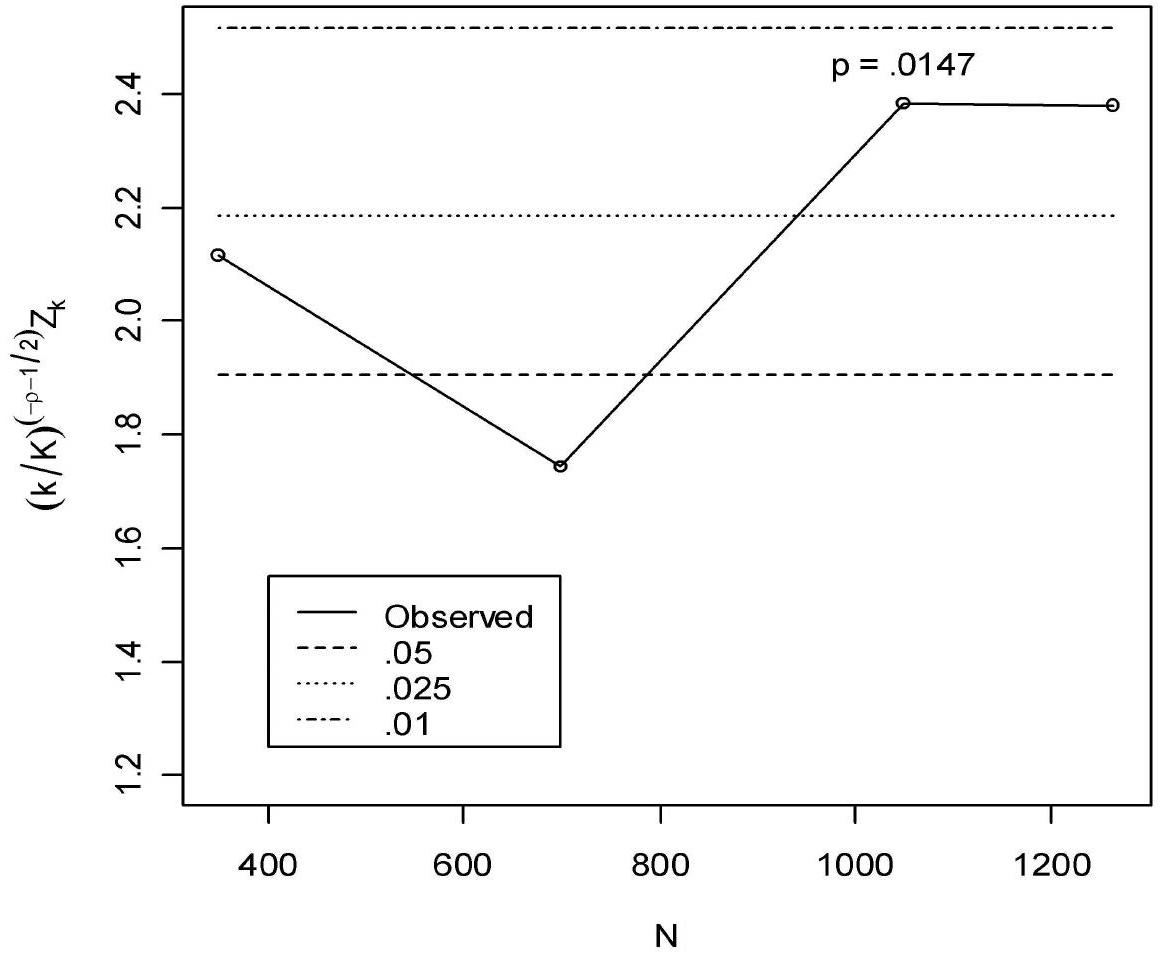
\includegraphics[alt={},max width=\textwidth]{94f53dbd-43ab-4208-a589-759d7fe17b97-37_955_1158_480_394}
\end{center}
\end{figure}

was used in the study. Here we consider a Wang-Tsiatis boundary with $\rho=.35$ to mimic the original boundary.

For the binomial interim data we use the cumulative data, estimated event rates and variances within each treatment group, and then compute a $Z$ -statistic using the difference in observed rates divided by its estimated standard error. Since there was an overrun, the final analysis had to weight the final $1267-1050=217$ patients as if they were the original 350 planned for the final enrollment cohort. This is done by using a weighted combination of the $Z$-statistic at the third interim and the final 217 patients. For $\rho=.35$, $(k / 4)^{-(.35-.5)} Z_{k}$ for $k=1,2,3,4$ are 2.1156, 1.7423, 2.3800, and 2.3771. The test statistic at the end of the trial is the maximum of these, and thus, $q_{4}=$ 2.3800. The sequential $p$-values are . 0299 .0299, .0147, and .0147. The sample\\
path $(k / 4)^{-(.35-.5)} Z_{k}$ for $k=1,2,3,4$ is plotted in Figure 1 along with the boundary lines for significance levels .01, .025, and .05.

A dip in the sample path is clearly seen in Figure 1, which suggests heterogeneity and warrants a closer examination. The stage-wise observed event rates for treatment and control are (.08, .17), (.13, .14), (.10, .16), and (.14, .17) for stage 1, 2, 3, and 4, respectively. There are no visible signs of qualitative heterogeneity, meaning that the treatment could be worse than the control. A formal overall test is not suggestive of a strong evidence for heterogeneity (Cochran's $Q$ chi-square is 3.16 with 3 degrees of freedom, for which the $p$ value is .37). The final repeated $p$-value of Jennison and Turnbull (p. 202, 2002) is $p=0.0148$. Thus, a significant final sequential $p$-value, $p=.0147$, can be interpreted as strong evidence to support the claim that the treatment is more effective than the control in reducing the overall event rate for the primary endpoint.

Heterogeneity in treatment effect can also cause difficulty for monitoring a trial. For illustration, suppose the Pocock boundary for the significance level $\alpha=.025$ were used. In Figure 2, the sample path $Z_{k}$ for $k=1,2,3,4$ is plotted along with boundary lines for significance levels .01, . 025 and .05. The boundary line for $\alpha=.025$ were crossed at the first interim analysis, suggesting a large treatment effect. If the DSMB took a cautious approach to require further confirmation of early results, the decision would be to continue to the second interim analysis. To their surprise, $Z_{2}$ dropped at the second interim. A test for heterogeneity after 2 interim analyses yields a $p$-value . 1 (with Cochran's $Q$ Chi-square being 2.78 with 1 degree of freedom), which is nominally significant according to the conventional significance level . 1 for interactions. If the trial were to stop at the second interim analysis, it would

\begin{figure}[h]
\begin{center}
\captionsetup{labelformat=empty}
\caption{Figure 2: Sample path for $\rho=.5$}
  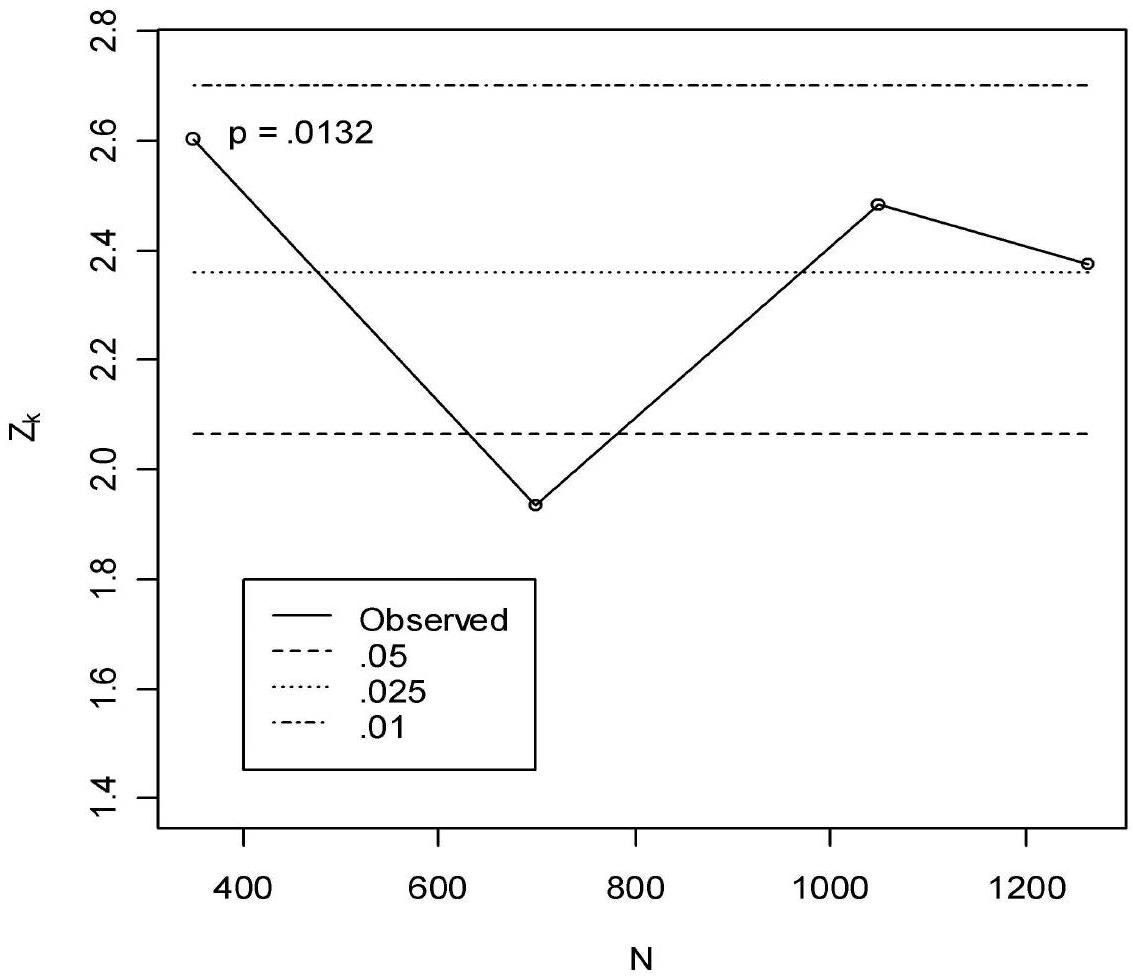
\includegraphics[alt={},max width=\textwidth]{94f53dbd-43ab-4208-a589-759d7fe17b97-39_977_1133_457_419}
\end{center}
\end{figure}

be difficult to interpret the sequential $p$-values and to further make a claim on the treatment effect. The DSMB might then decide to continue the trial to the third interim analysis and to finish the trial with a final analysis to account for over-running, again with 1, 267 patients. The treatment effect seen at the first interim is repeated at the third interim analysis. Following the same data examination as in the previous paragraph, the significant final $p$-value, .0132, can be interpreted as supporting the same efficacy claim for the treatment.

This example with apparent early heterogeneity illustrates a reason why Pocock boundaries might seldom be recommended with classical group sequential designs. With adaptively extended group sequential designs, it is now possible to use less conservative boundaries such as the Pocock boundary while still maintaining interpretable trial results.

\section*{4 Improper $p$-Values}
\subsection*{4.1 Stage-wise Ordering}
The stage-wise ordering proposed by Fairbanks and Madsen (1982) is used by Tsiatis, Rosner and Mehta (1984) to calculate confidence intervals following a group sequential trial. It is the preferred ordering of Jennison and Turnbull (p. 180, 2000) and of Proschan, Lan, and Wittes (p. 126, 2006). Cook (2002) contends that $p$-values following the stage-wise ordering cannot meaningfully quantify the strength of evidence against the null hypothesis: the $p$-values at later stages are bounded below by $\alpha$ probabilities already spent, regardless of how much later test statistics exceed the boundary. Liu and Pledger (2006) point out that adaptively increasing sample size exacerbates this issue, as the resulting test statistics can have a high probability of exceeding the boundary by a large amount.

For clinical trials in general, the fundamental flaw of stage-wise ordering is that it does not define an ordering for the entire sample space where the full sample path can be truncated by any $\mathcal{F}$-measurable stopping time $\tau$. The stage-wise ordering proposed is defined only on the sub-sample space consisting of the boundary crossing time $\tau_{0}$ and test statistic $Z_{\tau_{0}}$. Restriction to the sub-sample space can have undesirable consequences. We provide the following practical case. A group sequential trial with a mortality/morbidity endpoint stops at the first interim analysis when the significance boundary is just crossed. The spent significance level for the first interim analysis is $\alpha_{1}=.01$. The overall $p$-value, say, $p_{s w}$, by the stage-wise ordering according to Jennison and Turnbull (p. 180, 2000) is .0098. However, it is discovered later by the adjudication committee that an event is incorrectly classified. A correction of\\
the data is made and the final test statistic no longer reaches the significance boundary, leading to the conclusion that the significance level $\alpha=.025$ is not achieved. Using the stage-wise ordering, it is not clear how to correct the overall $p$-value $p_{s w}$ because the sample point ( $\tau, Z_{\tau}$ ) is no longer in the subsample space specified by the pre-defined stopping time $\tau_{0}$. Here, a single event changes the $p$-value against the null hypothesis from being overwhelmingly significant, with $p_{s w}=.0098$, to being not significant at the $\alpha=.025$ significance level. Therefore, $p_{s w}$ cannot be meaningfully interpreted as a $p$-value. Can the stage-wise ordering be expanded to accommodate stopping without crossing a boundary? Whitehead (1992) proposes a $p$-value for "under-running", which is essentially a $p$-value calculated as if the trial were truncated at an early interim analysis. With the current example, the under-running $p$-value procedure contains the special case of Proschan, Lan and Wittes (p. 126, 2006) that "if the trial is stopped at the first look, the $p$-value is the same as for a trial with no monitoring." According to Whitehead (1992) or Proschan, Lan and Wittes (2006), the $p$-value for the corrected data is .011, which is larger than the spent type I error rate of $\alpha_{1}=.01$ but still much smaller than the specified significance level of $\alpha=.025$. Thus, the $p$-value contradicts the criterion that the overall $p$-value is less than or equal to $\alpha$ if and only if the group sequential test crosses the significance boundary. Therefore, there is no obvious remedy to extend stage-wise ordering to any stopping time $\tau$.

We now illustrate other undesirable features of a $p$-value procedure defined through stage-wise ordering. In Brannath, Posch and Bauer (2002), an overall $p$-value is defined for a modified Fisher's combination test. The overall $p$-value is then used in a recursive combination test for multistage adaptive designs. Consider the two-stage combination test using Fisher's product $p_{1} p_{2}$ where $p_{1}$\\
and $p_{2}$ are the nominal $p$-values for the first and second stage. For given early decision boundaries $\alpha_{1}$ and $\alpha_{0}$ with $0 \leq \alpha_{1}<\alpha<\alpha_{0} \leq 1$, the null hypothesis is rejected at the first stage if $p_{1} \leq \alpha_{1}$; the trial stops for futility if $p_{1}>\alpha_{0}$; the trial continues to the second stage if $\alpha_{1}<p_{1} \leq \alpha_{0}$, and the null is rejected if $p_{1} p_{2} \leq c$ where the critical value $c=\left(\alpha-\alpha_{1}\right) /\left\{\log \left(\alpha_{0}\right)-\log \left(\alpha_{1}\right)\right\}$ is given by their equation (3). It is also assumed that $\alpha_{1}$ and $\alpha_{0}$ are carefully chosen so that $c \leq \alpha_{1}$. Applying the stage-wise ordering, they derived an overall $p$-value $p=p\left(p_{1}, p_{2}\right)$ in their equation (5), which is

$$
p\left(p_{1}, p_{2}\right)= \begin{cases}p_{1} & \text { if } p_{1} \leq \alpha_{1} \text { or } p_{1}>\alpha_{0} \\ \alpha_{1}+p_{1} p_{2}\left\{\log \left(\alpha_{0}\right)-\log \left(\alpha_{1}\right)\right\} & \text { if } p_{1} \in\left(\alpha_{1}, \alpha_{0}\right] \text { and } p_{1} p_{2} \leq \alpha_{1} \\ p_{1} p_{2}+p_{1} p_{2}\left\{\log \left(\alpha_{0}\right)-\log \left(p_{1} p_{2}\right)\right\} & \text { if } p_{1} \in\left(\alpha_{1}, \alpha_{0}\right] \text { and } p_{1} p_{2}>\alpha_{1}\end{cases}
$$

Now consider testing against the null hypothesis at a significance level $\mu$ that is smaller than $\alpha_{1}$. Then by definition, $p\left(p_{1}, p_{2}\right) \leq \mu$ if and only if $p_{1} \leq \mu$. As the test $p_{1} \leq \mu$ uses only $p_{1}$, it ignores the second stage data $p_{2}$. Thus, the test violates the intent-to-treatment principle. This contradicts the standard practice to use more data, not less data, for testing at a smaller significance level. Note that this undesirable feature also applies to the stage-wise $p$-value procedure in Jennison and Turnbull (p. 180, 2000), regardless of the underlying group sequential design.

In some situations, it is also more desirable to test against a null hypothesis at a larger significance level than originally planned. For example, a proof-of-concept (POC) trial for an experimental drug may be designed at the significance level $\alpha=.05$ with 80\%power. A new sponsor, upon acquisition of the drug, may decide to test against the null hypothesis at a large significance

\begin{figure}[h]
\begin{center}
\captionsetup{labelformat=empty}
\caption{Figure 3: Overall $p$-value for Fisher's Combination Test}
  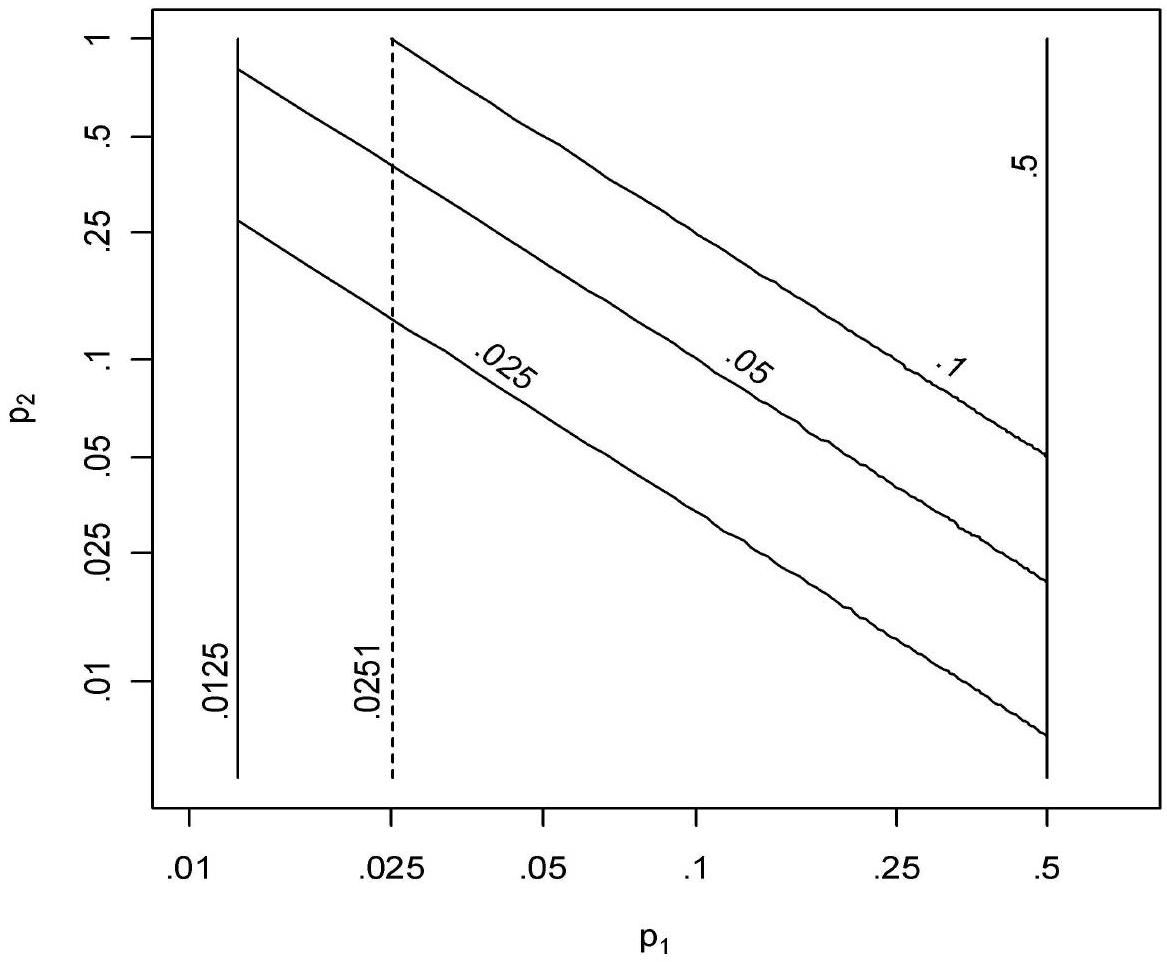
\includegraphics[alt={},max width=\textwidth]{94f53dbd-43ab-4208-a589-759d7fe17b97-43_962_1167_477_385}
\end{center}
\end{figure}

level, say, $\mu=.1$, in order to better control the type II error rate. This can be important for early development, as the type II error rate is the probability for abandoning the drug after the POC trial when the drug is, in fact, efficacious. Let us examine another difficulty when the overall $p$-value $p\left(p_{1}, p_{2}\right)$ is used to test against a null hypothesis at a larger significance level. For any $c^{\prime}>\alpha_{1}$ such that $\mu=c^{\prime}+c^{\prime}\left\{\log \left(\alpha_{0}\right)-\log \left(c^{\prime}\right)\right\}<\alpha_{0}$, it is easily shown that, for $p_{1} \in\left(\alpha_{1}, \alpha_{0}\right]$, rejecting the null hypothesis by $p\left(p_{1}, p_{2}\right) \leq \mu$ is equivalent to rejecting the null by either $p_{1} p_{2} \leq \alpha_{1}$ or $\alpha_{1}<p_{1} p_{2} \leq c^{\prime}$. But, for $p_{1} \in\left(\alpha_{1}, c^{\prime}\right]$, $p_{1} p_{2} \leq \alpha_{1}$ or $\alpha_{1}<p_{1} p_{2} \leq c^{\prime}$ is true for all $p_{2} \in[0,1]$.

We give the following numerical examples for the POC trial. Consider a design with $\alpha=.05, \alpha_{1}=.0125$ and $\alpha_{0}=.5$, for which $c=.0102<.0125=\alpha_{1}$. Let $c^{\prime}=.0251$, such that $\mu=c^{\prime}+c^{\prime}\left\{\log \left(\alpha_{0}\right)-\log \left(c^{\prime}\right)\right\}=.1<.5=\alpha_{0}$. Figure 3\\
shows how two $p$-values are combined. The axes are on a log scale; thus, contours of $p\left(p_{1}, p_{2}\right)$ are represented by straight lines. The solid vertical lines are drawn at $\alpha_{1}=.0125$ and $\alpha_{0}=.5$. Note that for $\mu \leq .0125, p\left(p_{1}, p_{2}\right) \leq \mu$ if and only if $p_{1} \leq \mu$, which does not use $p_{2}$. The diagonal lines represent equal products for $p_{1}$ and $p_{2}$. Values of $p_{1}$ between the . 0125 line and the dashed . 0251 line represent cases where the trial would continue past the first analysis but would result in $p\left(p_{1}, p_{2}\right)<.05$ regardless of $p_{2}$. For example, for $p_{1}=.015$, which is larger than $\alpha_{1}=.0125$ and smaller than $c^{\prime}=.0251$ and $\alpha_{0}=.5$, the null hypothesis is not rejected at the first stage because $p_{1}>\alpha_{1}$. For the second stage, let $p_{2}=.2$. Then $p_{1} p_{2}=.003<.0125=\alpha_{1}$. By Brannath, Posch and Bauer (2002), $p(.015, .2)=.0236<.1=\mu$. For $p_{2}=.99$, $p(.015, .99)=.0672<.1=\mu$. For $p_{2}=1$, which corresponds to the case that no data from the second stage are collected, $p(.015,1)=.0676<.1=\mu$.

These examples demonstrate the contradiction that the underlying null hypothesis cannot be rejected at the end of the first stage because the significance criterion, i.e., $p_{1} \leq \alpha_{1}$, is not met, yet the null hypothesis is rejected in the second stage without the need for any data. This contradiction is known as non-stochastic curtailing by Brannath, Posch and Bauer (2002). To exclude this for the $\alpha$-level test, they require that $\alpha_{1}$ and $\alpha_{0}$ be selected such that $c \leq \alpha_{1}$. However, there are other significance levels $\mu$, say, $\mu=.1$, for which their test $p\left(p_{1}, p_{2}\right) \leq \mu$ still induces non-stochastic curtailing. Thus, $p\left(p_{1}, p_{2}\right)$ by Brannath, Posch and Bauer (2002) is not an appropriate overall $p$-value. Although we have not made further investigation, we suspect that the recursive combination test procedure, which is based on recursive applications of $p\left(p_{1}, p_{2}\right)$, would exacerbate the issues we have identified.

\subsection*{4.2 Partial Likelihood-Based Orderings}
The three likelihood-based orderings by $Q_{\rho}(\underline{\omega})$ for $\rho=1,1 / 2$ or 0 proposed in Section 3.1 incorporate the totality of data, represented by the sample path $\underline{\omega}=\left\{\tau ; Z_{1}, \cdots, Z_{\tau}\right\}$. The three partial likelihood-based orderings by $(\tau / K)^{-(\rho-1 / 2)} Z_{\tau}$ for $\rho=1,1 / 2$ or 0 use only the terminal data $\left\{\tau ; Z_{\tau}\right\}$. Each of the partial likelihood-based orderings is well defined for the entire sample space, consisting of all possible sample paths of the form $\underline{\omega}=\left\{\tau ; Z_{1}, \cdots, Z_{\tau}\right\}$, as it is a binary relation over the sample space that is reflexive, antisymmetric, and transitive (see \href{http://www.Wikipedia.org}{www.Wikipedia.org} on partial order). However, it appears that $p$-value procedures proposed in the literature are only defined on a subsample space for which $\tau$ is restricted to $\tau_{0}$ at which a boundary is just crossed. From our literature review, we find that $\tau_{0}$ is used in Chang (1989), Emerson and Fleming (1990), Jennison and Turnbull (p. 179, 2000), Hall and Liu (2002), Cook (2002), and Gillen and Emerson (2005). There are two interesting exceptions. We are not able to find an explicit definition for a stopping time in the book by Proschan, Lan, and Wittes (2006). However, $\tau_{0}$ is implicitly used in their Examples 7.1 and 7.3 (pp. 118 and 121, 2006). We are surprised that the stopping time in Rosner and Tsiatis (1988) is not defined at all.

We now demonstrate that restriction to $\tau_{0}$ leads to improper $p$-values. Consider only the ordering by $(\tau / K)^{-(\rho-1 / 2)} Z_{\tau}$ for a given $\rho$. Let $b_{k}$ for $k=$ $1,2, \cdots, K$ be any boundary values computed to satisfy equation (1) for a group sequential test. Let $r$ be an observed value of $(\tau / K)^{-(\rho-1 / 2)} Z_{\tau}$ when $\tau=\tau_{0}$. Following Proschan, Lan, and Wittes (pp. 121 and 122, 2006), the $p$-value is given by


\begin{align*}
p(r)= & P_{\Delta=0}\left\{\left(\tau_{0} / K\right)^{-(\rho-1 / 2)} Z_{\tau_{0}} \geq r\right\} \\
= & P_{\Delta=0}\left\{Z_{\tau_{0}} \geq\left(\tau_{0} / K\right)^{\rho-1 / 2} r\right\} \\
= & P_{\Delta=0}\left[\bigcup_{k=1}^{K}\left\{\tau_{0}=k\right\} \cap\left\{Z_{k} \geq(k / K)^{\rho-1 / 2} r\right\}\right] \\
= & P_{\Delta=0}\left[Z_{1} \geq \max \left\{(1 / K)^{\rho-1 / 2} r, b_{1}\right\}\right] \\
& +\sum_{k=2}^{K-1} P_{\Delta=0}\left[\cap_{j=1}^{k-1}\left\{Z_{j}<b_{j}\right\} \cap\left\{Z_{k} \geq \max \left\{(k / K)^{\rho-1 / 2} r, b_{k}\right\}\right\}\right] \\
& +P_{\Delta=0}\left[\cap_{j=1}^{K-1}\left\{Z_{j}<b_{j}\right\} \cap\left\{Z_{K} \geq r\right\}\right] . \tag{15}
\end{align*}


Apart from the fact that the $p$-value procedure by equation (15) uses only partial data, we further demonstrate that it also causes monitoring and inferential difficulties when such a $p$-value is compared with a different significance level. We then demonstrate that the $p$-value procedure cannot be applied with an arbitrary stopping time $\tau$. For this purpose, it suffices to consider only the case with $K=2$, for which equation (15) reduces to


\begin{equation*}
p(r)=P_{\Delta=0}\left[Z_{1} \geq \max \left\{(1 / 2)^{\rho-1 / 2} r, b_{1}\right\}\right]+P_{\Delta=0}\left\{Z_{1}<b_{1}, Z_{2} \geq r\right\} . \tag{16}
\end{equation*}


We present numerical results for the MLE ordering for which $\rho=1$. First, consider monitoring an ongoing trial at a different significance level, say, $\mu=$ .01. Assume that when the trial is designed for $\alpha=.025$, the natural Wang-Tsiatis boundary values $b_{1}=(1 / 2)^{1 / 2} C_{\alpha}=1.9774$ and $b_{2}=C_{\alpha}=2.7965$ with $\rho=1$ are used. The rejection region of the group sequential test for $\alpha=.025$ is shown in Figure 4, which is the region on the right side of the . 025 vertical line plus the region above the . 025 horizontal line. Note that, according to equation (16), the $p$-values are identical, both equaling . 025 with $r=C_{\alpha}=2.7965$ regardless of whether $\tau_{0}=1$ or 2. For $\tau_{0}=1, Z_{1}$ just hits the boundary value $b_{1}=1.9774$, and for $\tau_{0}=2, Z_{2}$ just hits $b_{2}=2.7965$. In

\begin{figure}[h]
\begin{center}
\captionsetup{labelformat=empty}
\caption{Figure 4: Rejection Region for the MLE Ordering}
  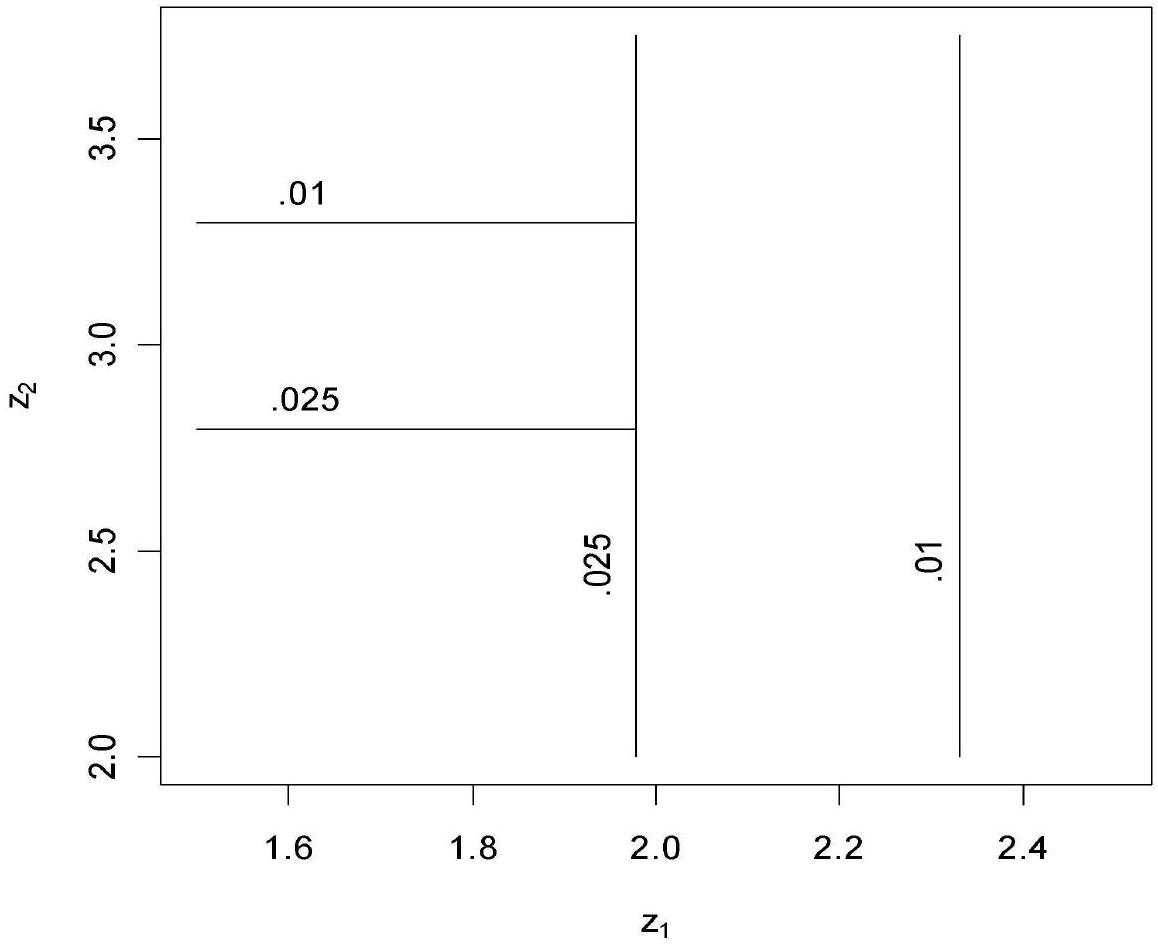
\includegraphics[alt={},max width=\textwidth]{94f53dbd-43ab-4208-a589-759d7fe17b97-47_946_1158_489_387}
\end{center}
\end{figure}

fact, this is generally true for any $r \geq C_{\alpha}$. Thus, $p$-values by equation (15) or (16) are similar to the $p$-values given by equation (14) in that $p$-values for boundary values are identical.

Now for $\mu=.01$, the critical value $r_{.01}$ such that $p\left(r_{.01}\right)=.01$ by equation (16) is $r_{.01}=3.2959$, for which the null hypothesis is rejected at the interim analysis if and only if $Z_{1} \geq(1 / 2)^{1 / 2} r_{.01}=2.3306=b_{1}^{\dagger}$, and the null hypothesis is rejected at the final analysis if and only if $Z_{1}<b_{1}=1.9774$ and $Z_{2} \geq r_{.01}=3.2959$. This two-stage test is illustrated graphically in figure 4, where the rejection region consists of the region on the right side of the . 01 vertical line and the top region bounded by the . 025 vertical line and . 01 horizontal line. The null hypothesis is not rejected in the region between the . 025 and . 01 vertical lines. This is the most interesting point that highlights the\\
inappropriateness of $p$-values by equations (15) and (16).\\
For $\alpha=.025$, the original boundary value $b_{1}=1.9774$ for the interim analysis serves the dual purposes of stopping the trial early and testing significance: the trial can stop at the interim analysis and reject the null hypothesis if and only if $Z_{1} \geq 1.9774=b_{1}$. For $\mu=.01$, the boundary value $b_{1}=1.9774$ no longer plays the role of a significance test, rather it is only used to stop the trial early. For this reason, we call $b_{1}=1.9774$ the monitoring boundary value and $b_{1}^{\dagger}=2.3306$ the significance boundary value. The discrepancy between the monitoring and significance boundary values, i.e., $b_{1}=1.9774$ and $b_{1}^{\dagger}=2.3306$, causes monitoring and inferential difficulties. If the trial stops at the interim analysis according to $Z_{1} \geq b_{1}=1.9774$, then the null hypothesis cannot be rejected unless $Z_{1} \geq b_{1}^{\dagger}=2.3306$; if the trial continues according to $Z_{1}<b_{1}^{\dagger}=2.3306$, then the null hypothesis at the final analysis cannot be rejected at $\mu=.01$ level, even for extremely large $Z_{2}$, unless $Z_{1}<b_{1}=1.9774$. If the final test $Z_{2} \geq r_{.01}=3.2959$ ignores $Z_{1}<b_{1}=1.9774$, the type I error rate is .0241, which is inflated above $\mu=.01$.

What if we apply equation (16) when the trial stops at the first interim analysis even though the boundary is not crossed? Assume that the O'BrienFleming (Wang-Tsiatis with $\rho=0$ ) boundary values $b_{1}=(1 / 2)^{-1 / 2} C_{\alpha}=$ 2.7965 and $b_{2}=C_{\alpha}=1.9774$ are used originally in the design for $\alpha=.025$. We still use the $p$-value given by equation (16) for the partial likelihood ordering with $\rho=1$. Let the observed $Z_{1}$ be $r=(1 / 2)^{1 / 2} C_{\alpha}=1.3983$, which is smaller than $b_{1}=2.7965$. Applying equation (16) with $\rho=1$ for the MLE ordering, we obtain $p=.025$, by which the null hypothesis should be rejected. However, this is not correct, since the original boundary value $b_{1}=2.7965$ is not crossed. This is a contradiction with the basic principle that the overall\\
$p$-value is significant at $\alpha=.025$ if and only if the null hypothesis is rejected by the group sequential test. Thus, $p$-values by equation (16) cannot be applied for any stopping time $\tau$.

Notice that in the two previous examples, the boundary values $b_{1}$ and $b_{2}$ are 1.9774 and 2.7965 for $\rho=1$, and 2.7965 and 1.9774 for $\rho=0$. In general, if $E\left\{Z_{k}\right\}=0, \operatorname{Var}\left\{Z_{k}\right\}=1$ for $k=1,2$, and $\operatorname{Cov}\left\{Z_{1}, Z_{2}\right\}=\sigma_{12}$, then $P\left\{Z_{1}>b_{1}, Z_{2}>b_{2}\right\}=g\left(\sigma_{12}, b_{1}, b_{2}\right)$, which is a bivariate normal probability function. Because a bivariate normal distribution as such is symmetric, we also have $P\left\{Z_{1}>b_{2}, Z_{2}>b_{1}\right\}=g\left(\sigma_{12}, b_{1}, b_{2}\right)$. In the example above with $\rho=1$, we must have $b_{1}=2^{-1 / 2} b_{2}$ while, with $\rho=0$, we must have $b_{2}=2^{1 / 2} b_{1}$. In both cases we solve for the bound using $g\left(\sigma_{12}, r, 2^{-1 / 2} r\right)=.025$, which explains the coincidence of the boundary values $b_{1}$ and $b_{2}$ being swapped from $\rho=1$ to $\rho=0$.

Finally, for the other two partial likelihood-based orderings with $\rho=1 / 2$ or 0, similar numerical examples are available from the authors.

\section*{Acknowledgments}
We would like to thank the editor for his suggestion to publish a supplemental paper at the amstat web site. We would also like to thank two referees and an associate editor for pointing out that our original manuscript overlooked some of the existing literature. Without the latter, we would not have conducted further research of all existing orderings in the literature, and, consequently, would not have discovered various issues with all existing likelihood orderings. Last but not least, we would like to thank Emily Anderson and Jennifer Liu for their assistance in final editing, and Cynthia Gilchrist for obtaining copies of many references.

\section*{References}
\begin{itemize}
  \item[1.] Armitage, P., Freeman, P. R., et al. (1989). Discussion of 'Interim analyses: The repeated confidence interval approach' (by Jennison, C., and Turnbull, B. W.). Journal of the Royal Statistical Society, Series B, 51, 334, 339.
  \item[2.] Armitage, P., McPherson, C. K., and Rowe, B. C. (1969). Repeated significance tests on accumulating data. Journal of the Royal Statistical Society, Ser. A, 132, 235-244.
  \item[3.] Billingsley, P. (1986). Probability and Measure. 2nd Ed., New York: Wiley \& Sons.
  \item[4.] Barndorff-Nielsen, O. E., and Cox, D. R. (1994). Inference and Asymptotics. London: Chapman \& Hall.
  \item[5.] Brannath, W., Posch, M. and Bauer, P. (2002). Recursive combination tests. Journal of the American Statistical Association 97, 236-244.
  \item[6.] The CAPTURE Investigators. (1997). Randomized placebo-controlled trial of abciximab before and during coronary intervention in refractory unstable angina: the CAPTURE study.", Lancet, 349, 1429-1435.
  \item[7.] 21 CFR 312.21.\\
\href{http://www.accessdata.fda.gov/scripts/cdrh/cfdocs/cfcfr/}{http://www.accessdata.fda.gov/scripts/cdrh/cfdocs/cfcfr/}\\
CFRSearch.cfm?fr=312.21
  \item[8.] Chang, M. N. (1989). Confidence intervals for a normal mean following a group sequential test. Biometrics, 45, 247-254.
  \item[9.] Cook, R. J. (1996). Coupled error spending functions for parallel bivariate sequential tests. Biometrics, 52, 442-450.
\end{itemize}

\begin{itemize}
  \item[10.] Cook, R. J., and Farewell, V. T. (1994). Guidelines for monitoring efficacy and toxicity responses in clinical trials. Biometrics, 50, 1146-1152.
  \item[11.] Cook, T. D. (2002). $P$-value adjustment in sequential clinical trials. Biometrics, 58, 1005-1011.
  \item[12.] Cox, D.R., and Hinkley, D.V. (1974). Theoretical Statistics. Chapman \& Hall, London.
  \item[13.] Cui, L., Hung, H. M. J., and Wang, S. J. (1999). Modification of sample size in group sequential clinical trials. Biometrics, 55, 853-857.
  \item[14.] Cytel Software Corporation. (2007). EaSt 5, Cambridge, Mass.
  \item[15.] Davis, C. E. (1997). Secondary endpoints can be validly analyzed, even if the primary endpoint does not provide clear statistical significance. Controlled Clinical Trials, 18, 557-560.
  \item[16.] Ellenberg, S. S., Fleming, T. R., and DeMets, D. L. (2002). Data Monitoring Committees in Clinical Trials, A Practical Perspective, West Sussex, United Kingdom: Wiley.
  \item[17.] Emerson, S. S., and Fleming, T. R. (1990). Parameter estimation following group sequential hypothesis testing. Biometrika, 77, 875-892.
  \item[18.] Fairbanks, K., and Madsen, R. (1982). $P$-values for tests using a repeated significance test design. Biometrika, 69, 69-74.
  \item[19.] Fisher, L. (1998). Self-designing clinical trials. Statistics in Medicine, 17, 1551-1562.
  \item[20.] Follmann, D. A., Proschan, M. A., and Geller, N. L. (1994). Monitoring pairwise comparisons in multi-armed clinical trials. Biometrics, 50, 325-336.
\end{itemize}

\begin{itemize}
  \item[21.] Gillen, D. L., and Emerson, S. S. (2005). A note on $p$-values under group sequential testing and nonproportional hazards. Biometrics, 61, 546-551.
  \item[22.] Hacking, I. (1965). Logic of Statistical Inference. Cambridge: University Press.
  \item[23.] Hall, W. J., and Liu, A. (2002). Sequential tests and estimators after overruning based on maximum-likelihood ordering. Biometrika, 89, 699-707.
  \item[24.] Jennison, C., and Turnbull, B. W. (1993). Group sequential tests for bivariate response: Interim analyses of clinical trials with both efficacy and safety endpoints. Biometrics, 49, 741-752.
  \item[25.] Jennison, C., and Turnbull, B. W. (2000). Group Sequential Methods with Applications to Clinical Trials, Boca Raton: Chapman \& Hall.
  \item[26.] Jennison, C., and Turnbull, B. W. (2003). Mid-course sample size modification in clinical trials based on the observed treatment effect. Statistics in Medicine, 22, 971-993.
  \item[27.] Lan, K. K. G., and DeMets, D. L. (1983). Discrete sequential boundaries for clinical trials. Biometrika, 70, 659-663.
  \item[28.] Laska, E. M., and Meisner, M. J. (1989). Testing whether an identified treatment is best. Biometrics, 45, 1139-1151.
  \item[29.] Liu, Q., and Anderson, K. M. (2008). On adaptive extensions of group sequential trials for clinical investigations. Revision submitted to Journal of the American Statistical Association.
  \item[30.] Liu, Q., Anderson, K. M. and Pledger, G. W. (2004). Benefit-risk evaluation of multi-stage adaptive designs. Sequential Analysis, 23, 317-331.
\end{itemize}

\begin{itemize}
  \item[31.] Liu, Q., and Chi, G. Y. H. (2001). On sample size and inference for two-stage adaptive designs. Biometrics 57, 172-177.
  \item[32.] Liu, Q., and Pledger, G. W. (2006). On design and inference for twostage adaptive clinical trials with dependent data. Journal of Statistical Planning and Inference, 136, 1962-1984.
  \item[33.] Liu, Q., Proschan, M. A., and Pledger, G. W. (2002). A unified theory of two-stage adaptive designs. Journal of the American Statistical Association, 97, 1034-1041.
  \item[34.] Marcus, R., Peritz, E., and Gabriel, K. R. (1976). On closed testing procedures with special reference to ordered analysis of variance. Biometrika, 63, 655-660.
  \item[35.] Müller, H., and Schäfer, H. (2001). Adaptive group sequential designs for clinical trials: Combining the advantages of adaptive and of classical group sequential approaches. Biometrics, 57, 886-891.
  \item[36.] O'Brien, P. C. (1984). Procedures for comparing samples with multiple endpoints. Biometrics, 40, 1079-1087.
  \item[37.] O'Neill, R. T. (1997). Secondary endpoints cannot be validly analyzed if the primary endpoint does not demonstrate clear statistical significance. Controlled Clinical Trials, 18, 550-556.
  \item[38.] Prentice, R. L. (1997). Discussion: On the role and analysis of secondary outcomes in clinical trials. Controlled Clinical Trials, 18, 561-567.
  \item[39.] Proschan, M. A., Liu, Q., and Hunsberger, S. A. (2003). Practical midcourse sample size modification in clinical trials. Controlled Clinical Trials, 24, 4-15.
  \item[40.] Proschan, M. A., Lan, K. K. G., and Wittes, J. T. (2006). Statistical Monitoring of Clinical Trials, New York: Springer.
\end{itemize}

\begin{itemize}
  \item[41.] Rosner, G. L., and Tsiatis, A. A. (1988). Exact confidence intervals following a group sequential trial: A comparison of methods. Biometrika, 75, 723-729.
  \item[42.] Tang, D., and Geller, N. L. (1999). Closed testing procedures for group sequential trials with multiple endpoints. Biometrics, 55, 1188-1192.
  \item[43.] Tang, D., Geller, N. L., and Pocock, S. J. (1993). On the design and analysis of randomized clinical trials with multiple endpoints. Biometrics, 49, 23-30.
  \item[44.] Tang, D., Gnecco, C., and Geller, N. L. (1989). Design of group sequential clinical trials with multiple endpoints. Journal of the American Statistical Association, 84, 776-779.
  \item[45.] Tsiatis, A. A., and Mehta, C. (2003). On the inefficiency of the adaptive design for monitoring clinical trials. Biometrika, 90, 367-378.
  \item[46.] Tsiatis, A. A., Rosner, G. L., and Mehta, C. R. (1984). Exact confidence intervals following a group sequential test. Biometrics, 40, 797-803.
  \item[47.] Wang, S. K., and Tsiatis, A. A. (1987). Approximately optimal oneparameter boundaries for group sequential trials. Biometrics, 43, 193-200.
  \item[48.] Whitehead, J. (1986). Supplementary analysis at the conclusion of a sequential clinical trial. Biometrics, 42, 573-581.
  \item[49.] Whitehead, J. (1992). Overrunning and underrunning in sequential clinical trials. Controlled Clinical Trials, 13, 106-121.
  \item[50.] Women's Health Initiative Manuals. vol. 1. Study Protocol and Policies, Seattle: WHI Clinical Coordinating Center, Fred Hutchinson Cancer Research Center, (1994).
\end{itemize}

\end{document}
